\documentclass[a4paper]{article}
\usepackage{cmap}
\usepackage[utf8]{inputenc}
\usepackage[T2A]{fontenc}
\usepackage[english,russian]{babel} 
\usepackage[left=15mm, top=15mm, right=15mm, bottom=42mm, nohead, nofoot]{geometry}
\usepackage{blindtext}  % рыба-текст
\usepackage{graphicx}  % изобржаения
\usepackage{float} % плавающие объекты
\usepackage{wrapfig}  % изобржаения
\usepackage{tikz} % графика
\usepackage{mdframed} % рамки
\usepackage{xcolor} % определение цветов
\usepackage{nicefrac} % красивые дроби
\usepackage{cancel} % сокращение
\usepackage{amsmath,amsfonts,amssymb} % математический пакет
\usepackage{hyperref}  % гиперссылки
\usepackage{fancybox,fancyhdr} % хедер и футер
\usepackage{listings} % код
\pagestyle{fancy}
\fancyhf{}
\fancyhead[L]{Лабораторная работа №3}
\fancyhead[R]{\textit{Фильтрация и выделение контуров}}
\fancyfoot[C]{\thepage}
\headsep=8mm
\footskip=20mm

\definecolor{urlcolor}{HTML}{3454D1}
\definecolor{linkcolor}{HTML}{3454D1}
\hypersetup{pdfstartview=FitH, linkcolor=linkcolor, urlcolor=urlcolor, colorlinks=true}

\definecolor{strings}{rgb}{0,0.6,0}
\definecolor{comments}{rgb}{0,0.3,0}
\definecolor{numbers}{rgb}{0.5,0.5,0.5}
\definecolor{keywords}{rgb}{0.09,0.61,0.95}
\definecolor{background}{rgb}{0.97,0.97,0.97}
\lstdefinestyle{codestyle}{
    backgroundcolor=\color{background},
    commentstyle=\color{comments},
    keywordstyle=\color{keywords},
    stringstyle=\color{strings},
    numberstyle=\tiny\color{numbers},
    basicstyle=\ttfamily\footnotesize,
    breakatwhitespace=false,
    breaklines=true,
    captionpos=b,
    inputencoding=utf8,
    keepspaces=true,
    numbers=left,
    numbersep=5pt,
    showspaces=false,
    showstringspaces=false,
    showtabs=false,
    tabsize=2,
    extendedchars=true,
    literate=
    {а}{{\cyra}}1
    {б}{{\cyrb}}1
    {в}{{\cyrv}}1
    {г}{{\cyrg}}1
    {д}{{\cyrd}}1
    {е}{{\cyre}}1
    {ж}{{\cyrzh}}1
    {з}{{\cyrz}}1
    {и}{{\cyri}}1
    {й}{{\cyrishrt}}1
    {к}{{\cyrk}}1
    {л}{{\cyrl}}1
    {м}{{\cyrm}}1
    {н}{{\cyrn}}1
    {о}{{\cyro}}1
    {п}{{\cyrp}}1
    {р}{{\cyrr}}1
    {с}{{\cyrs}}1
    {т}{{\cyrt}}1
    {у}{{\cyru}}1
    {ф}{{\cyrf}}1
    {х}{{\cyrh}}1
    {ц}{{\cyrc}}1
    {ч}{{\cyrch}}1
    {ш}{{\cyrsh}}1
    {щ}{{\cyrshch}}1
    {ъ}{{\cyrhrdsn}}1
    {ы}{{\cyrery}}1
    {ь}{{\cyrsftsn}}1
    {э}{{\cyrerev}}1
    {ю}{{\cyryu}}1
    {я}{{\cyrya}}1
    {А}{{\CYRA}}1
    {Б}{{\CYRB}}1
    {В}{{\CYRV}}1
    {Г}{{\CYRG}}1
    {Д}{{\CYR96}}1
    {Е}{{\CYRE}}1
    {Ж}{{\CYRZH}}1
    {З}{{\CYRZ}}1
    {И}{{\CYRI}}1
    {Й}{{\CYRISHRT}}1
    {К}{{\CYRK}}1
    {Л}{{\CYRL}}1
    {М}{{\CYRM}}1
    {Н}{{\CYRN}}1
    {О}{{\CYRO}}1
    {П}{{\CYRP}}1
    {Р}{{\CYRR}}1
    {С}{{\CYRS}}1
    {Т}{{\CYRT}}1
    {У}{{\CYRU}}1
    {Ф}{{\CYRF}}1
    {Х}{{\CYRH}}1
    {Ц}{{\CYRC}}1
    {Ч}{{\CYRCH}}1
    {Ш}{{\CYRSH}}1
    {Щ}{{\CYRSHCH}}1
    {Ъ}{{\CYRHRDSN}}1
    {Ы}{{\CYRERY}}1
    {Ь}{{\CYRSFTSN}}1
    {Э}{{\CYREREV}}1
    {Ю}{{\CYRYU}}1
    {Я}{{\CYRYA}}1
}

\lstset{style=codestyle}

\addto\captionsrussian{
  \renewcommand{\contentsname}
    {\centering Содержание}
}
\newcommand{\addsection}[1]{
    \phantomsection
    \addcontentsline{toc}{section}{#1}
    \section*{\centering #1}
}
\newcommand{\addsubsection}[1]{
    \phantomsection
    \addcontentsline{toc}{subsection}{#1}
    \subsection*{\centering #1}
}
\newcommand{\addsubsubsection}[1]{
    \phantomsection
    \addcontentsline{toc}{subsubsection}{#1}
    \subsubsection*{\centering #1}
}

\newmdenv[
  leftmargin = 0.5em,
  skipabove = 0.5em,
  skipbelow = 0.5em,
  linewidth = 1pt,
  rightline = false,
  topline = false,
  bottomline = false
]{quotebox}

\newlength{\tempheight}
\newcommand{\Let}{
\mathbin{\text{\settoheight{\tempheight}{\mathstrut}\raisebox{0.4\pgflinewidth}{
\tikz[baseline=0.5ex,line cap=round,line join=round] \draw (0,0) --++ (0.3em,0) --++ (0,2.3ex) --++ (-0.3em,0);
}}}}
\newcommand*\squared[1]{\tikz[baseline=(char.base)]{
            \node[shape=rectangle,draw,inner sep=4pt] (char) {#1};}}
\newcommand*\msquared[1]{\tikz[baseline=(char.base)]{
            \node[shape=rectangle,draw,inner sep=4pt] (char) {$\displaystyle #1$};}}
\newcommand{\at}{\biggr\rvert}
\newcommand{\shiftright}[3]{\makebox[#2][r]{\makebox[#1][l]{#3}}}
\newcommand{\e}{\;\text{e}}
\let\oldint\int
\def\int{\oldint\limits}
\DeclareRobustCommand{\divby}{%
  \mathrel{\vbox{\baselineskip.65ex\lineskiplimit0pt\hbox{.}\hbox{.}\hbox{.}}}%
}

\newcommand\NB{\textbf{N\kern-0.32em\textcolor{red}{B}}}

\begin{document}
\begin{titlepage}
    \begin{center}
        Федеральное государственное автономное образовательное \\ учреждение высшего образования \\[6pt]
        САНКТ-ПЕТЕРБУРГСКИЙ НАЦИОНАЛЬНЫЙ \\ ИССЛЕДОВАТЕЛЬСКИЙ УНИВЕРСИТЕТ ИТМО \\[16pt]
        Факультет систем управления и робототехники \\[26em]
        Лабораторная работа №3 \\[0.5em]
        \textbf{ФИЛЬТРАЦИЯ И ВЫДЕЛЕНИЕ КОНТУРОВ}
    \end{center}\,\\[10em]
    \begin{flushright}
        Студенты: Овчинников П.А.\\
        Румянцев А.А.\\
        Чебаненко Д.А.\\[0.7em]
        Поток: ТЕХ.ЗРЕНИЕ 2.1 \\[0.7em]
        Преподаватель: Шаветов С.В.
    \end{flushright}\,\\[4.8em]
    \begin{center}
        {\small Санкт-Петербург \\ 2024}
    \end{center}
\end{titlepage}
\setcounter{page}{2}
\tableofcontents\newpage
\addsection{Цель работы}
В этой работе мы изучим разные типы шумов и фильтров. С помощью последних мы научимся фильтровать изображения от шумов. Также, используя фильтры, мы научимся выделять контуры в изображении. И всё это мы сможем сделать с помощью библиотек \verb|OpenCV|, \verb|scikit-image| и \verb|SciPy| прямо в \verb|Python|. Весь код будет приведён ссылкой на приватный гист в GitHub Gist, которую мы оставим в конце работы.\\[0.5em]
И перед её выполнением взглянем первый и последний раз на исходное изображение:
\begin{figure}[H]
    \centering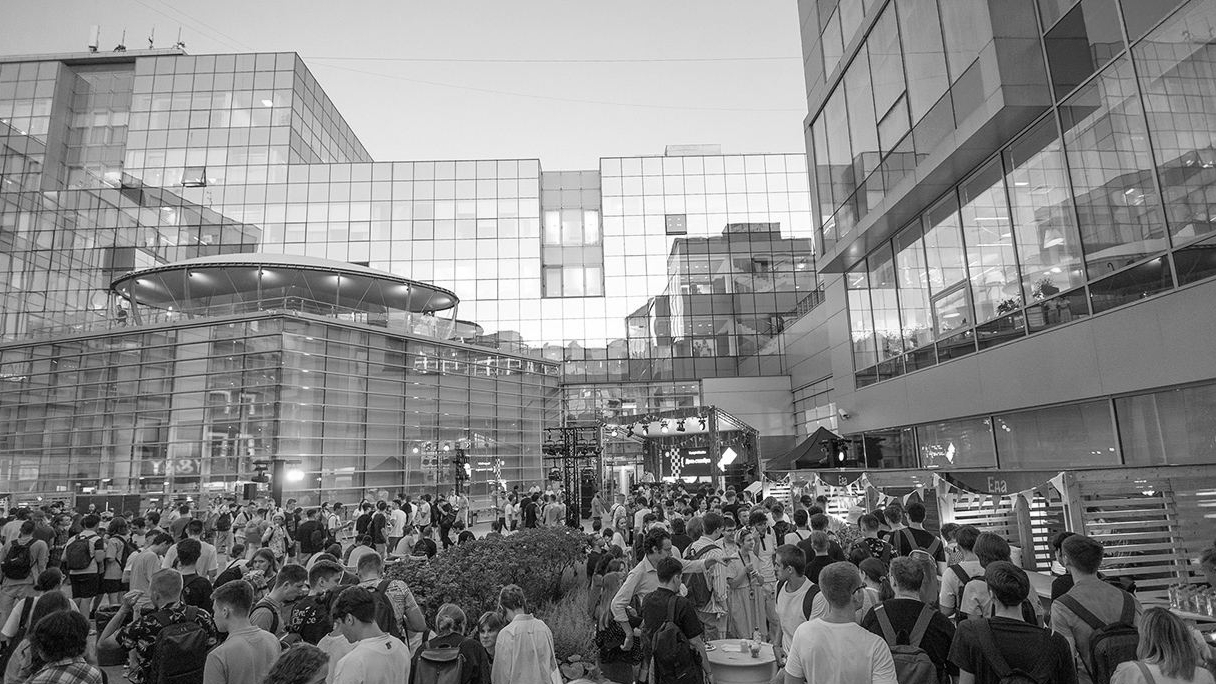
\includegraphics[width=0.7\textwidth]{images/photo.jpg}
    \caption{Исходное изображение}
\end{figure}

% MARK: Шумы
\addsection{Давайте пошумим!}
Итак, начнём с шумов. По каждому из них я приведу теоретическую справку и только затем покажу результат их применения к изображению, дабы сэкономить пространство.
% MARK: Импульсный шум
\addsubsection{Импульсный шум}
Первый, один из простых --- импульсный шум, появляющийся, например, из-за ошибок декодирования. Такой шум ещё называется точечным шумом, потому что приводит к появлению на изображении белых и чёрных точек, которые ещё называют «солью» и «перцем». И работает он очень просто:
$$I_n(x, y) = \begin{cases}
        d,       & \text{с вероятностью }p,       \\
        s_{x,y}, & \text{с вероятностью }(1 - p).
    \end{cases}$$
Здесь $s_{x,y}$ --- интенсивность пикселя исходного изображения, $I_n$ --- зашумлённое изображение, $p$ --- вероятность появления шума в пикселе, $d$ --- вероятность появления белой точки (чем выше, тем больше вероятность, что появится белая точка, иначе появится чёрная). Выходит, мы можем регулировать как вероятность появления шума в принципе, так и отношение «соли» к «перцу».
% MARK: Аддитивный шум
\addsubsection{Аддитивный шум}
Аддитивный шум предполагает наличие распределения функции плотности вероятности, которая просто добавляется к исходному изображению:
$$I_n(x, y) = I(x, y) + \eta(x, y).$$
$I$ --- исходная функция, $\eta$ --- аддитивный шум с гауссовым или любым другим распределением функции плотности вероятности, а $I_n$ --- зашумлённое изображение.\\
% MARK: Мультипликативный и спекл-шум
\addsubsection{Мультипликативный шум и спекл-шум}
Мультипликативный шум --- то же самое, что и аддитивный шум, но шум не добавляется к исходному изображению, а умножается на него. Зернистость плёнки или ультразвуковые изображение --- примеры такого шума.
$$I_n(x, y) = I(x, y) \cdot \eta(x, y)$$
Изображения, снятые медицинскими сканерами или радарами, обладают светлыми крапинками (спеклами), разделёнными тёмными участками изображения --- это частный случай мультипликативного шума, так называемый спекл-шум.
% MARK: Гауссов шум
\addsubsection{Гауссов шум}
Когда сцена недостаточно освещена или высокая температура в помещении плохо влияет на матрицу фотокамеры, появляется гауссов шум или нормальный шум. Именно этот шум в небольшом количестве появляется на фотографиях и от него обычно стараются избавиться. Функция распределения плотности вероятности $p(z)$ случайной величины z описывается следующим выражением:
$$p(z) = \frac{1}{\sigma\sqrt{2\pi}}\e^{\frac{-(z-\mu)^2}{2\sigma^2}},$$
где $z$ --- интенсивность изображения, $\mu$ --- среднее (или мат.ожидание) величины $z$, $\sigma$ --- среднеквадратичное отклонение.
% MARK: Шум квантования
\addsubsection{Шум квантования}
Шум квантования --- ошибки, возникающие при квантовании сигнала, когда сигнал округляется или усекается. Такой шум не устраняется, поэтому нужно быть очень осторожным, при квантовании изображения. Одно из точных приближение к шуму квантования --- распределение Пуассона, которое выглядит вот так:
$$p(z) = \frac{\lambda^z}{z!}\e^{-\lambda}.$$
Здесь $z$ --- так же интенсивность изображения, а $\lambda$ --- мат.ожидание величины.
\addsubsection{Применение шумов к изображению}
\begin{figure}[H]
    \begin{minipage}{0.49\textwidth}
        \centering 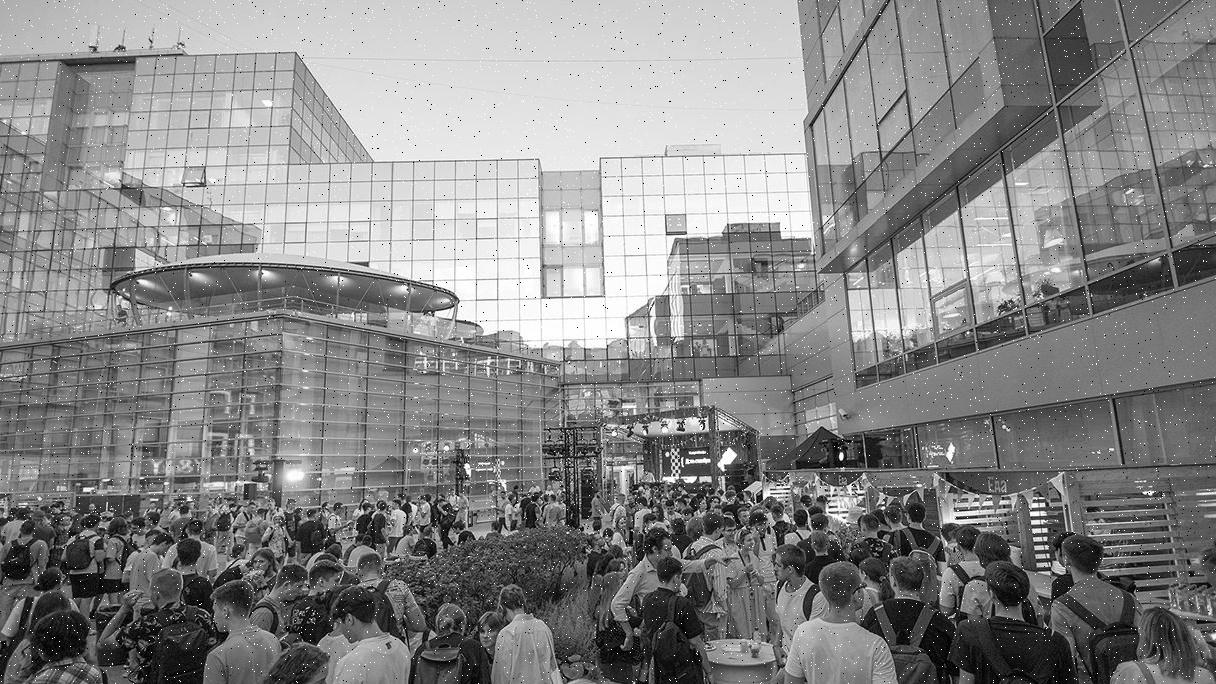
\includegraphics[width=\textwidth]{images/1_noise/impulse.jpg}
        \caption{Импульсный шум}
    \end{minipage}\hfill
    \begin{minipage}{0.49\textwidth}
        \centering 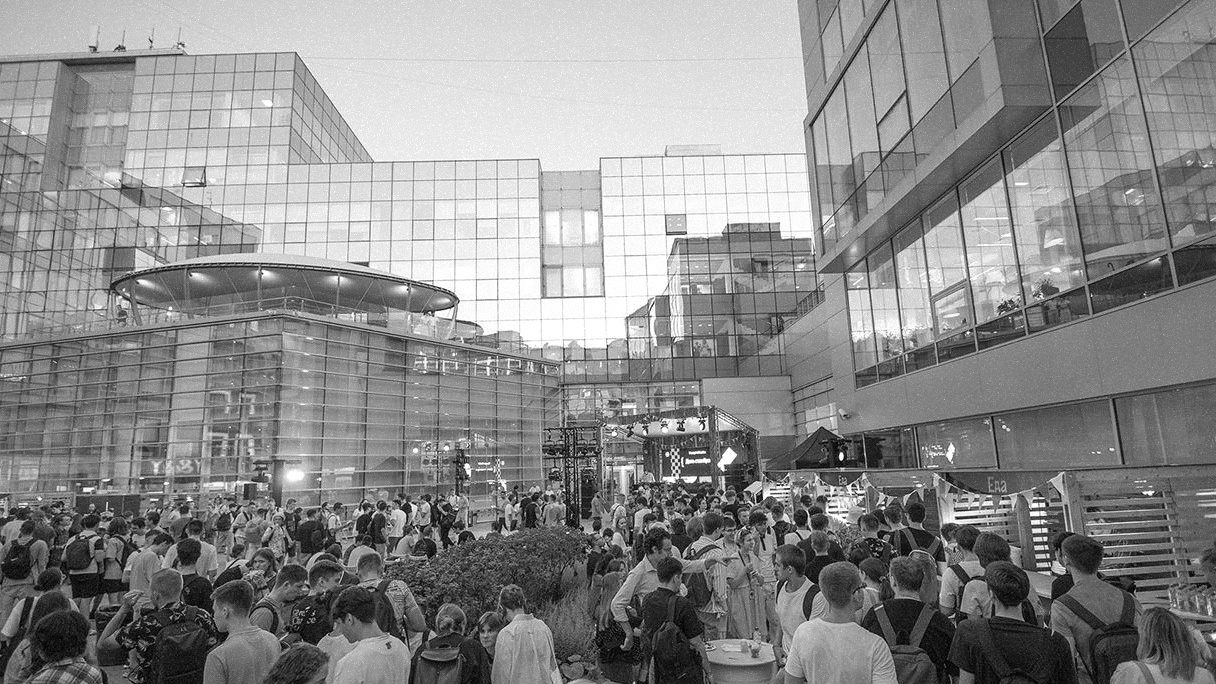
\includegraphics[width=\textwidth]{images/1_noise/additive.jpg}
        \caption{Аддитивный шум}
    \end{minipage}
\end{figure}
\begin{figure}[H]
    \begin{minipage}{0.49\textwidth}
        \centering 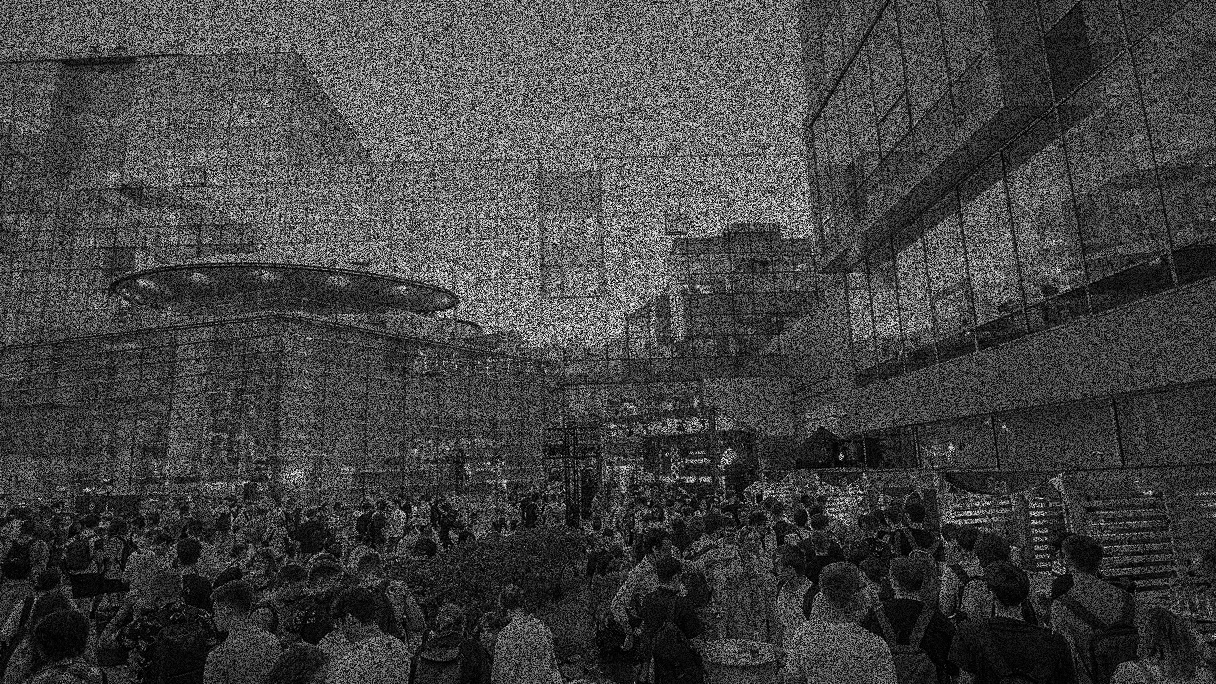
\includegraphics[width=\textwidth]{images/1_noise/multiplicative.jpg}
        \caption{Мультипликативный шум}
    \end{minipage}\hfill
    \begin{minipage}{0.49\textwidth}
        \centering 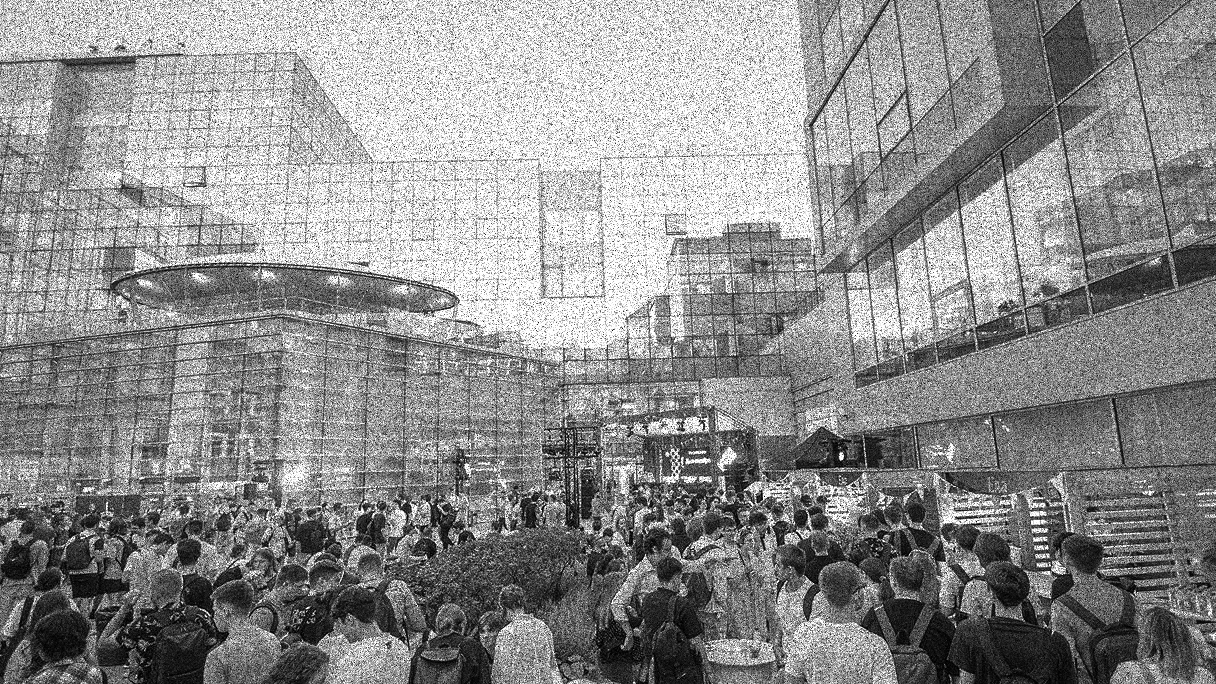
\includegraphics[width=\textwidth]{images/1_noise/speckle.jpg}
        \caption{Спекл-шум}
    \end{minipage}
\end{figure}
\begin{figure}[H]
    \begin{minipage}{0.49\textwidth}
        \centering 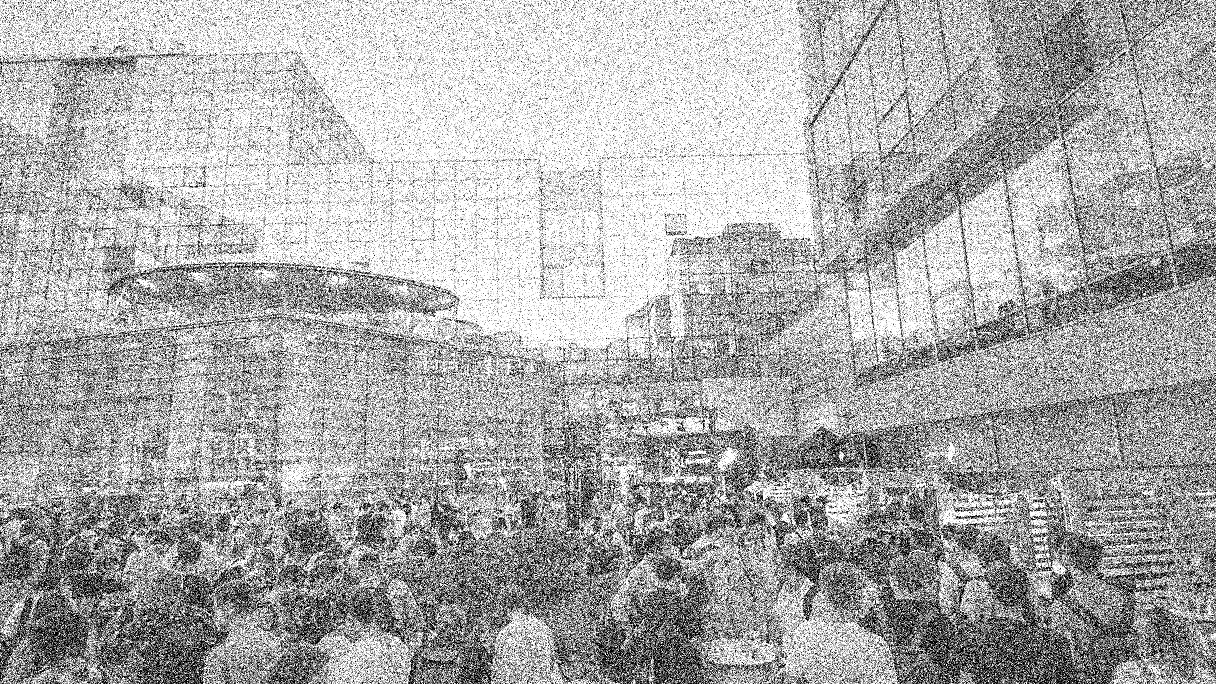
\includegraphics[width=\textwidth]{images/1_noise/gaussian.jpg}
        \caption{Гауссов шум}
    \end{minipage}\hfill
    \begin{minipage}{0.49\textwidth}
        \centering 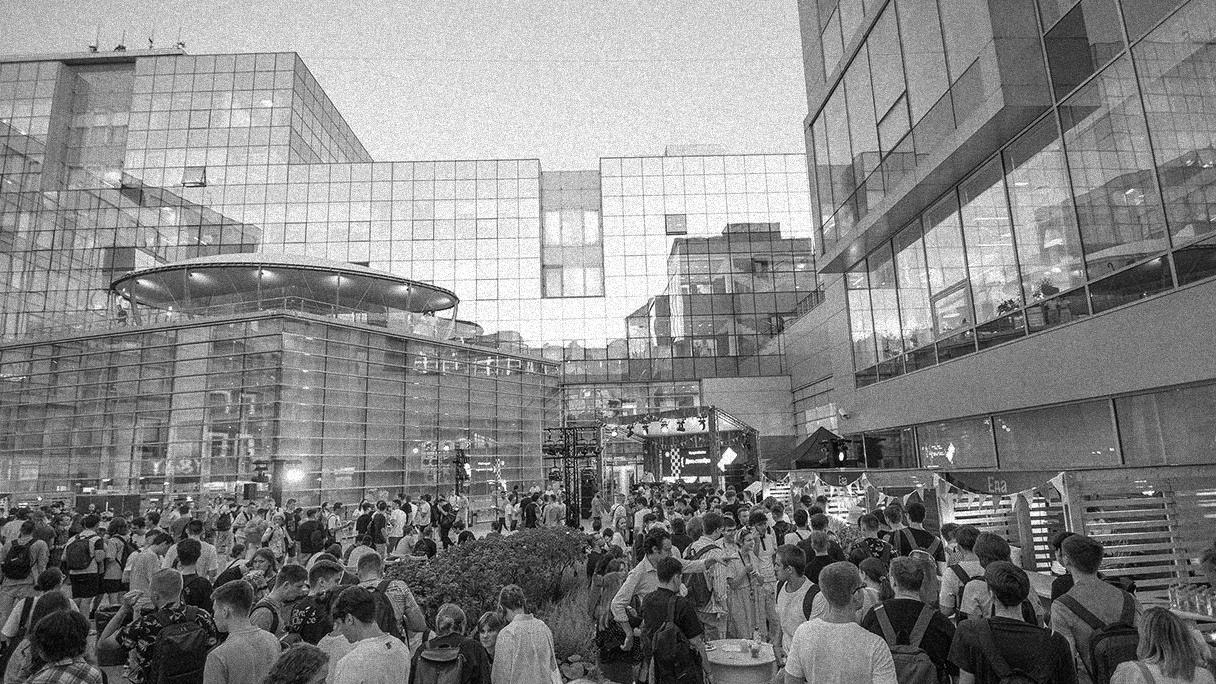
\includegraphics[width=\textwidth]{images/1_noise/poisson.jpg}
        \caption{Шум квантования}
    \end{minipage}
\end{figure}\,

% MARK: low-rate фильтры
\addsection{Низкочастотная фильтрация (или повесть «Прекращаем шуметь!»)}
Низкочастотные фильтры ослабляют высокочастотные компоненты (области с сильным изменением интенсивностей --- например, границы объектов) и оставляют низкочастотные компоненты без изменений. Именно такие фильтры снижают уровень шума, и в результате мы получаем сглаженное или размытое изображение.
% MARK: Фильтр Гаусса
\addsubsection{Фильтр Гаусса}
Один из простейших фильтров, который активно применяется во многих сферах и чаще известен как «размытие по Гауссу». Цифровые камеры многих смартфонов используют этот фильтр для ослабления шума, а некоторые графические приложения перед уменьшением размера изображения могут применить фильтр для предотвращения артефактов и алиасинга. И вот как выглядит двумерный фильтр Гаусса:
$$G_\sigma = \frac{1}{2\pi\sigma^2}\e^{-\frac{x^2+y^2}{2\sigma^2}} = \frac{1}{\sigma\sqrt{2\pi}}\e^{\frac{-x^2}{2\sigma^2}}\cdot\frac{1}{\sigma\sqrt{2\pi}}\e^{\frac{-y^2}{2\sigma^2}}$$
С ростом $\sigma$ изображение размывается сильнее.\newpage\noindent
Вот как фильтр Гаусса применяется к каждому из шумов (размера ядра $3\times3$):
\begin{figure}[H]
    \begin{minipage}{0.49\textwidth}
        \centering 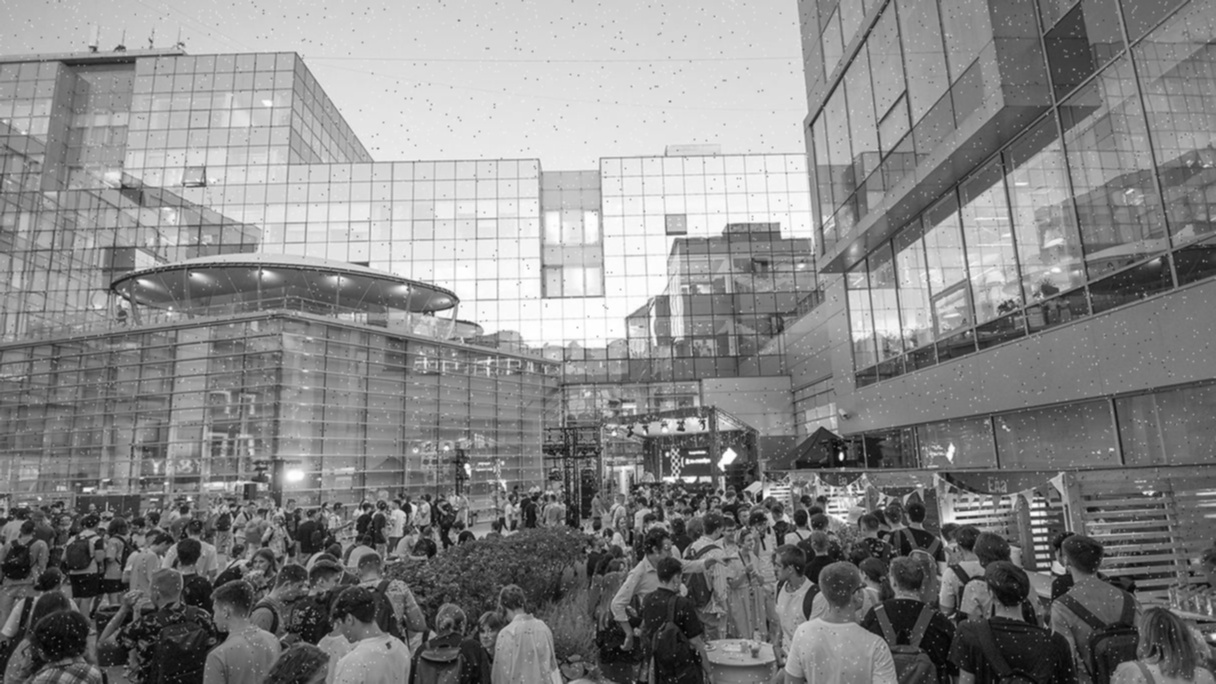
\includegraphics[width=\textwidth]{images/2_low_filters/impulse - gaussian (ksize=(3, 3), sigmaX=0).jpg}
        \caption{Импульсный шум + фильтр Гаусса}
    \end{minipage}\hfill
    \begin{minipage}{0.49\textwidth}
        \centering 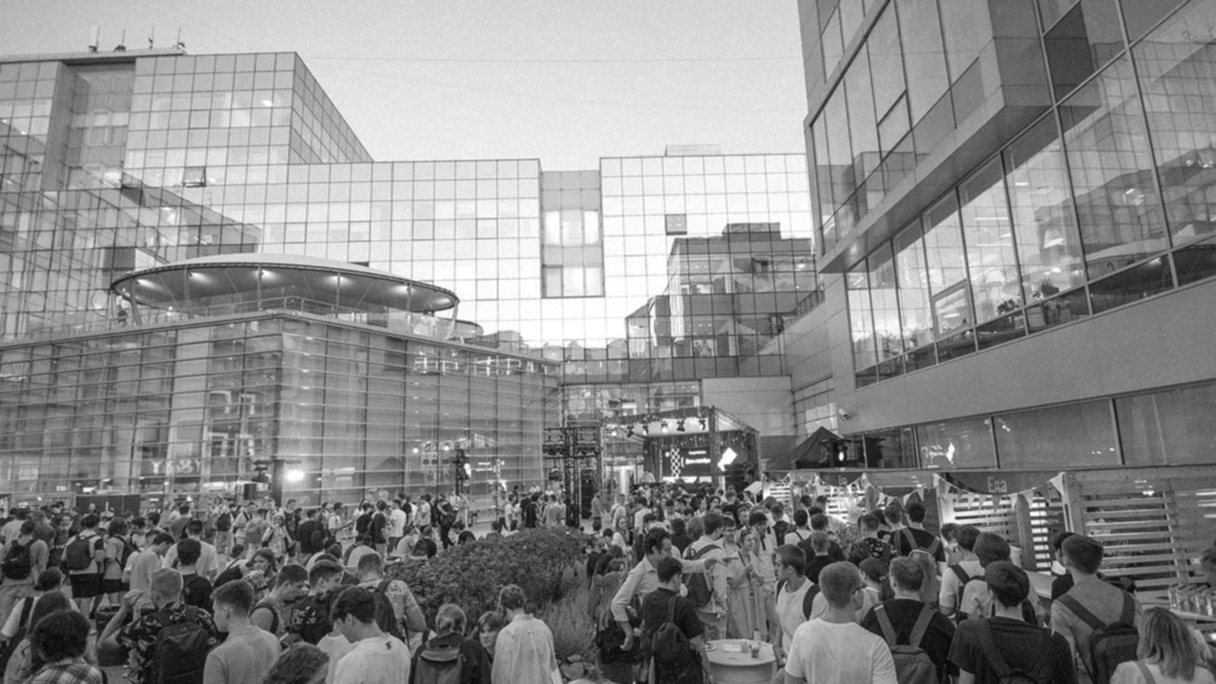
\includegraphics[width=\textwidth]{images/2_low_filters/additive - gaussian (ksize=(3, 3), sigmaX=0).jpg}
        \caption{Аддитивный шум + фильтр Гаусса}
    \end{minipage}
\end{figure}
\begin{figure}[H]
    \begin{minipage}{0.49\textwidth}
        \centering 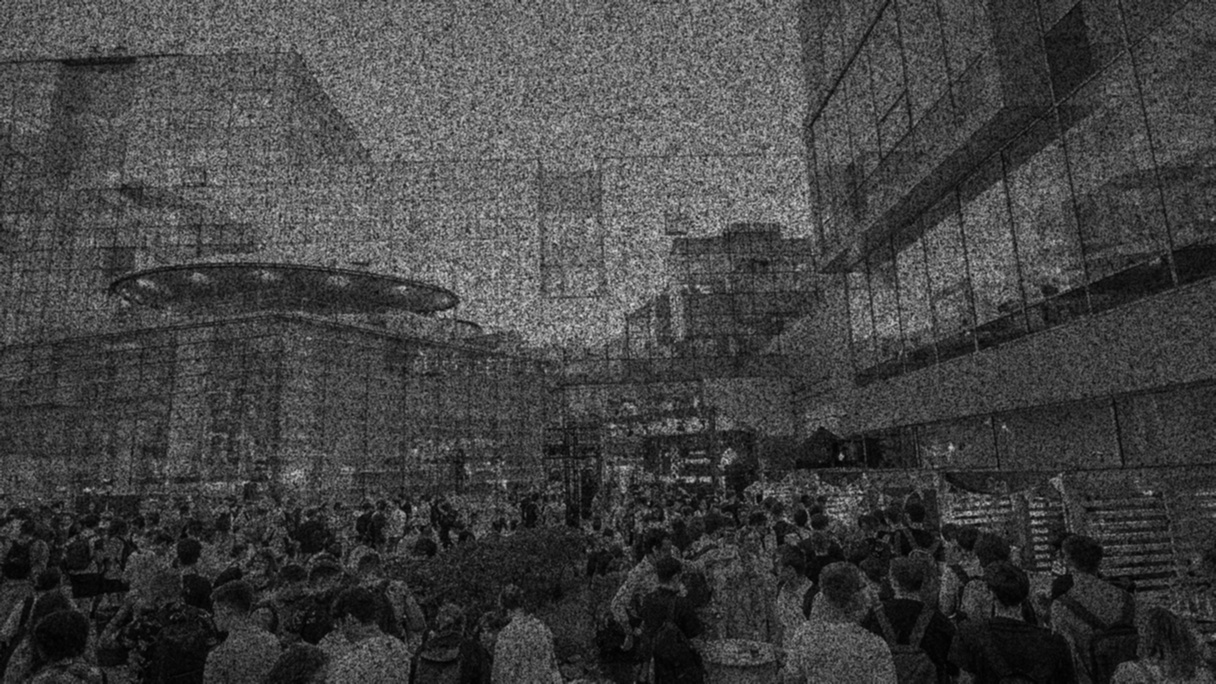
\includegraphics[width=\textwidth]{images/2_low_filters/multiplicative - gaussian (ksize=(3, 3), sigmaX=0).jpg}
        \caption{Мультипликативный шум + фильтр Гаусса}
    \end{minipage}\hfill
    \begin{minipage}{0.49\textwidth}
        \centering 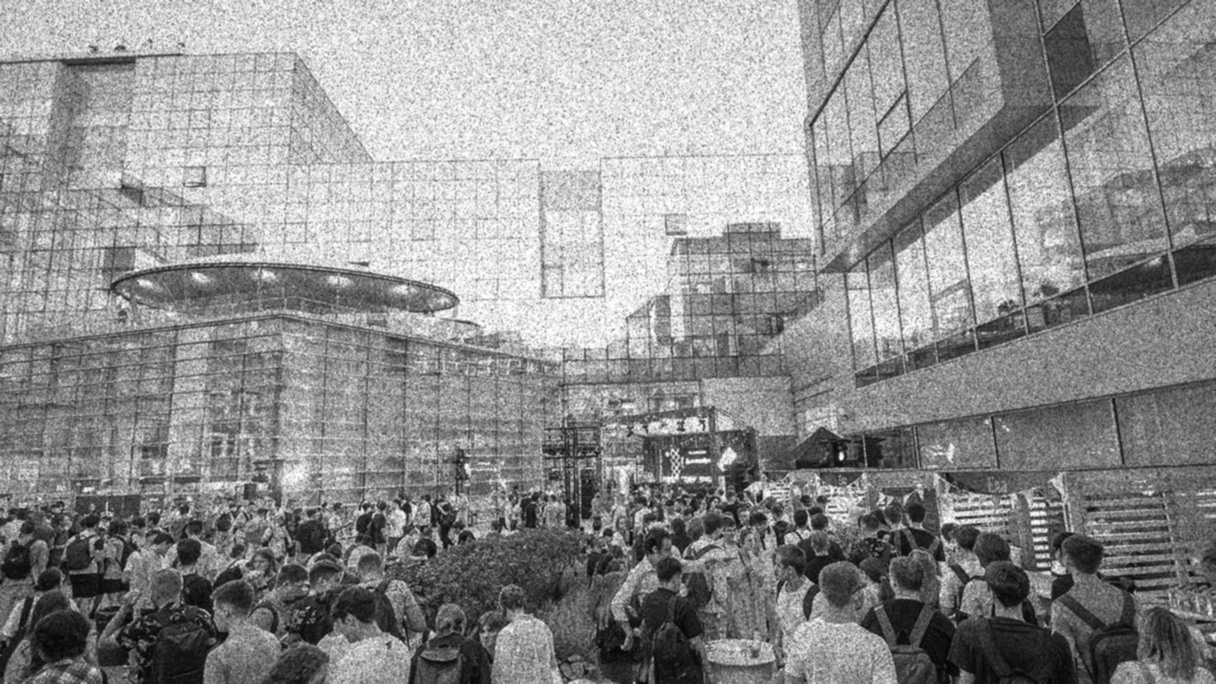
\includegraphics[width=\textwidth]{images/2_low_filters/speckle - gaussian (ksize=(3, 3), sigmaX=0).jpg}
        \caption{Спекл-шум + фильтр Гаусса}
    \end{minipage}
\end{figure}
\begin{figure}[H]
    \begin{minipage}{0.49\textwidth}
        \centering 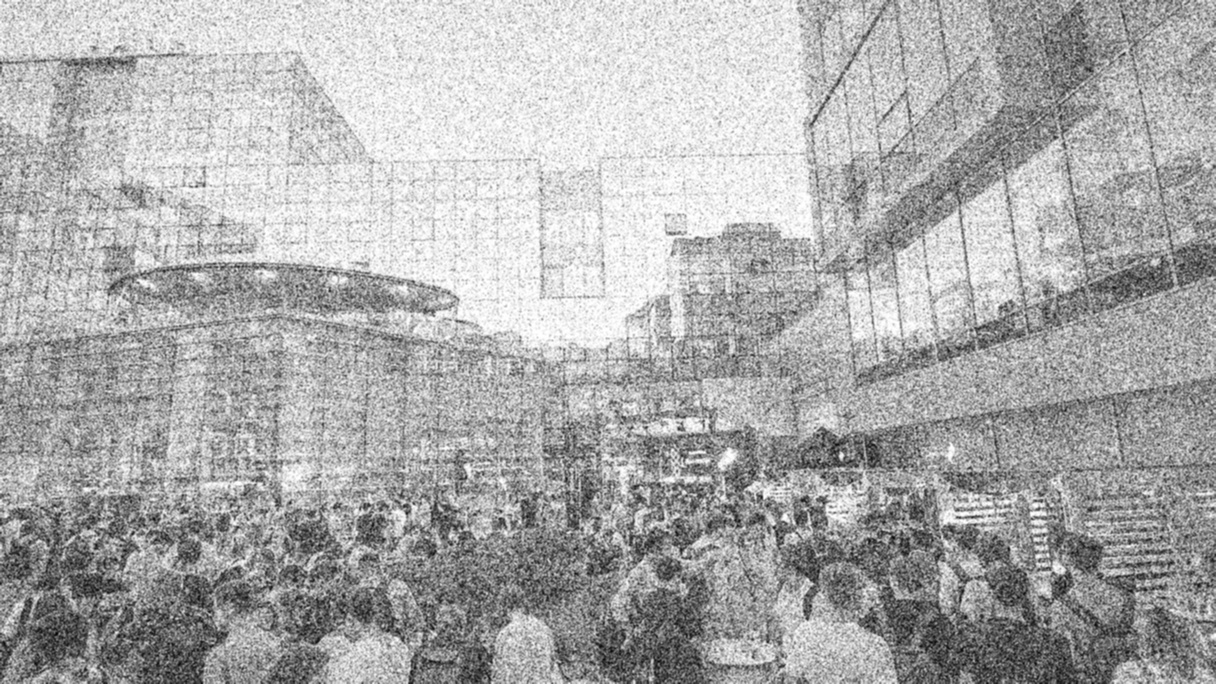
\includegraphics[width=\textwidth]{images/2_low_filters/gaussian - gaussian (ksize=(3, 3), sigmaX=0).jpg}
        \caption{Гауссов шум + фильтр Гаусса}
    \end{minipage}\hfill
    \begin{minipage}{0.49\textwidth}
        \centering 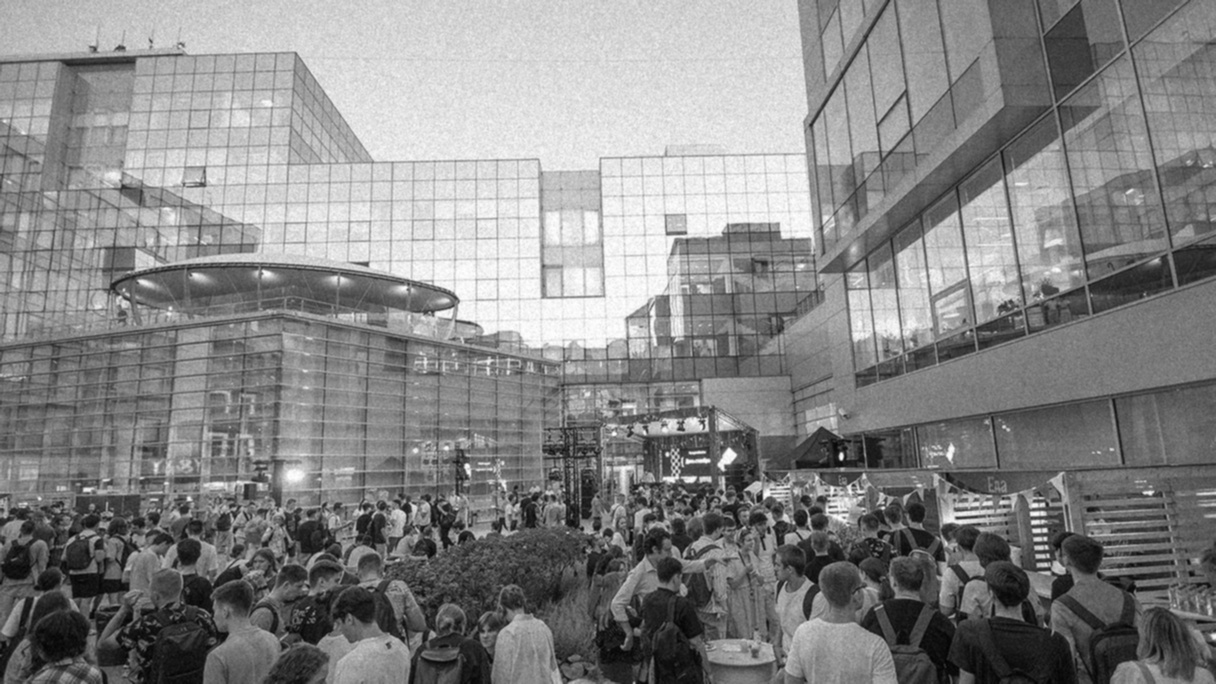
\includegraphics[width=\textwidth]{images/2_low_filters/poisson - gaussian (ksize=(3, 3), sigmaX=0).jpg}
        \caption{Шум квантования + фильтр Гаусса}
    \end{minipage}
\end{figure}
\noindent Как мы видим, фильтр Гаусса хорошо подавляет аддитивный шум.
% MARK: Контргармонический усредняющий фильтр
\addsubsection{Контргармонический усредняющий фильтр}
$$I_f(x, y) = \frac{\sum_{i=0}^m\sum_{j=0}^n I(i, j)^{Q+1}}{\sum_{i=0}^m\sum_{j=0}^n I(i, j)^{Q}}$$
$Q$ --- порядок фильтра. Контргармонический фильтр является обобщением усредняющих фильтров и может подавалять как шум типа «соль» ($Q < 0$), так и шум типа «перец» ($Q > 0$), но фильтр не способен удалить одновременно белые и чёрные точки.
\begin{figure}[H]
    \begin{minipage}{0.49\textwidth}
        \centering 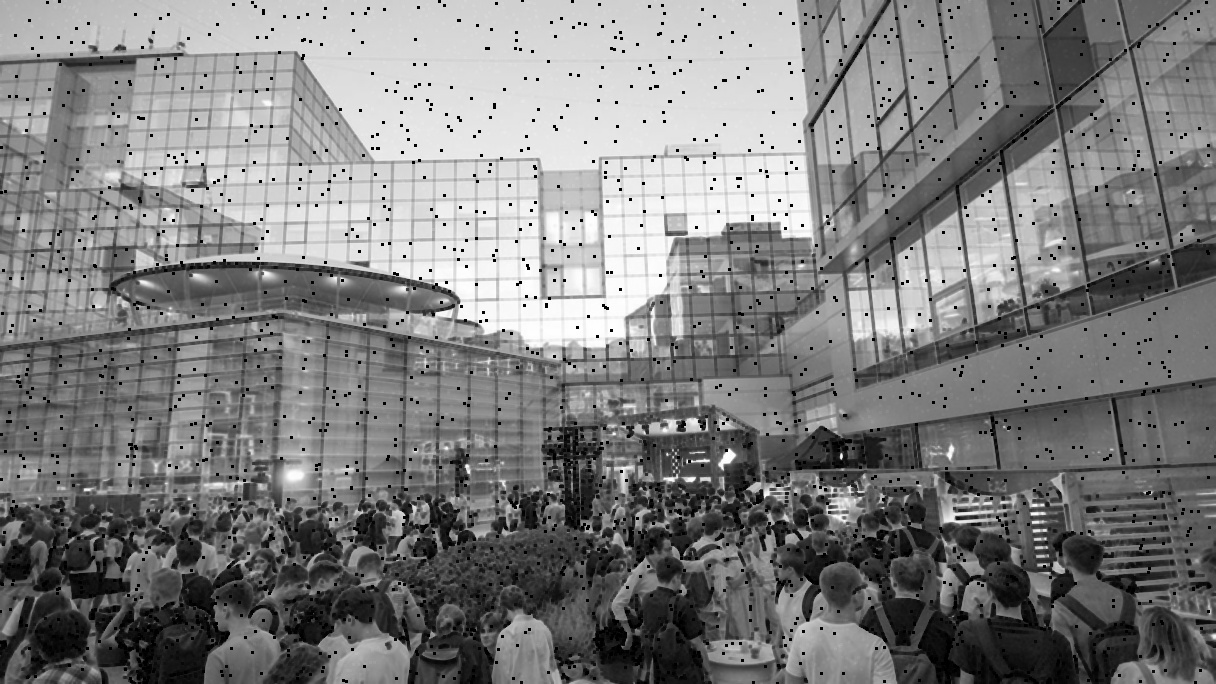
\includegraphics[width=\textwidth]{images/2_low_filters/impulse - contrharmonic (Q=-1.5).jpg}
        \caption{Импульсный шум + фильтр ($Q = -1.5$)}
    \end{minipage}\hfill
    \begin{minipage}{0.49\textwidth}
        \centering 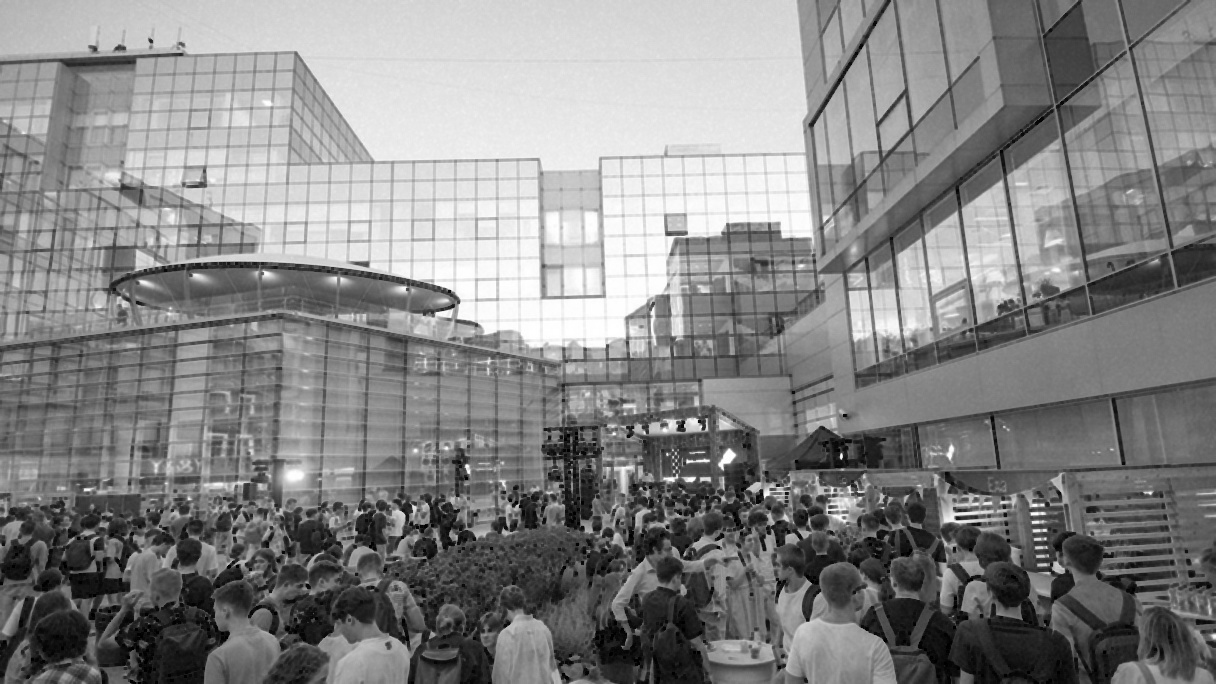
\includegraphics[width=\textwidth]{images/2_low_filters/additive - contrharmonic (Q=-1.5).jpg}
        \caption{Аддитивный шум + фильтр ($Q = -1.5$)}
    \end{minipage}
\end{figure}
\begin{figure}[H]
    \begin{minipage}{0.49\textwidth}
        \centering 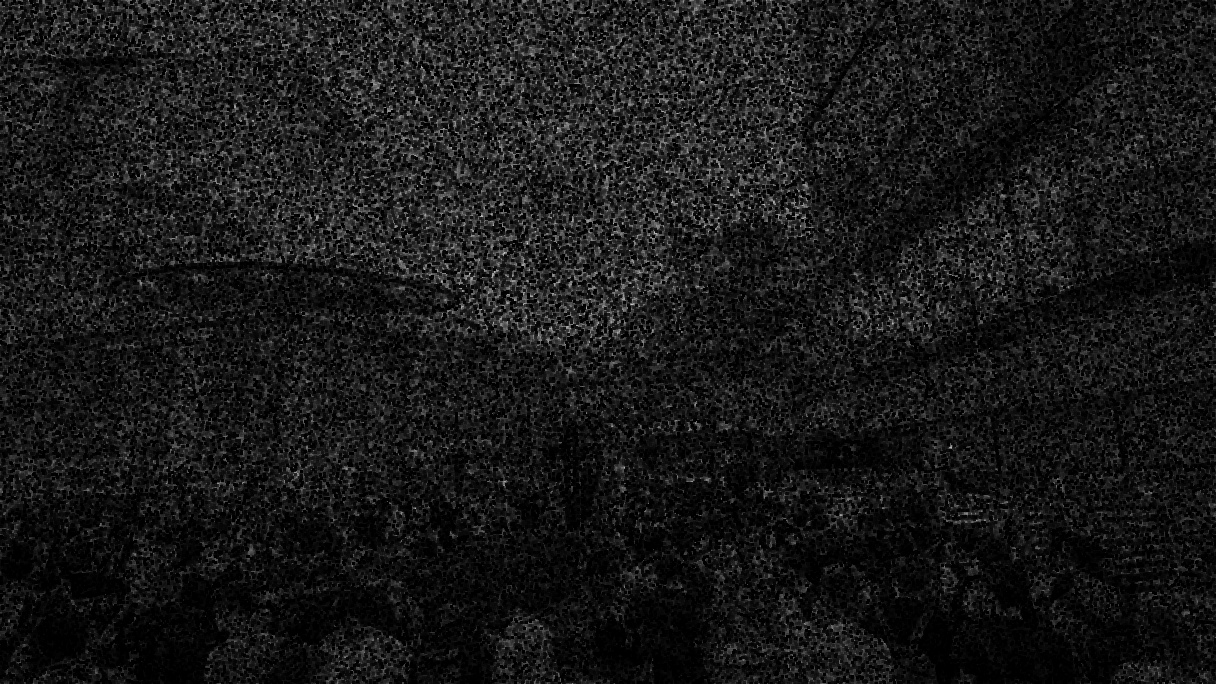
\includegraphics[width=\textwidth]{images/2_low_filters/multiplicative - contrharmonic (Q=-1.5).jpg}
        \caption{Мульти-ный шум + фильтр ($Q = -1.5$)}
    \end{minipage}\hfill
    \begin{minipage}{0.49\textwidth}
        \centering 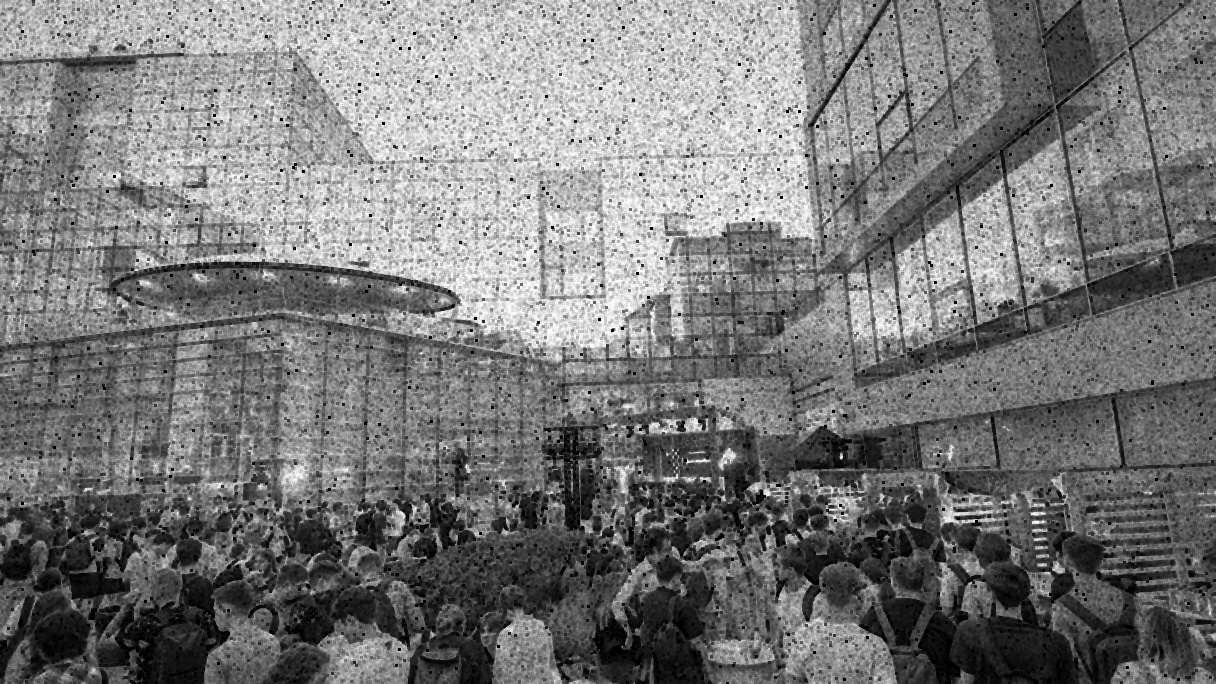
\includegraphics[width=\textwidth]{images/2_low_filters/speckle - contrharmonic (Q=-1.5).jpg}
        \caption{Спекл-шум + фильтр ($Q = -1.5$)}
    \end{minipage}
\end{figure}
\begin{figure}[H]
    \begin{minipage}{0.49\textwidth}
        \centering 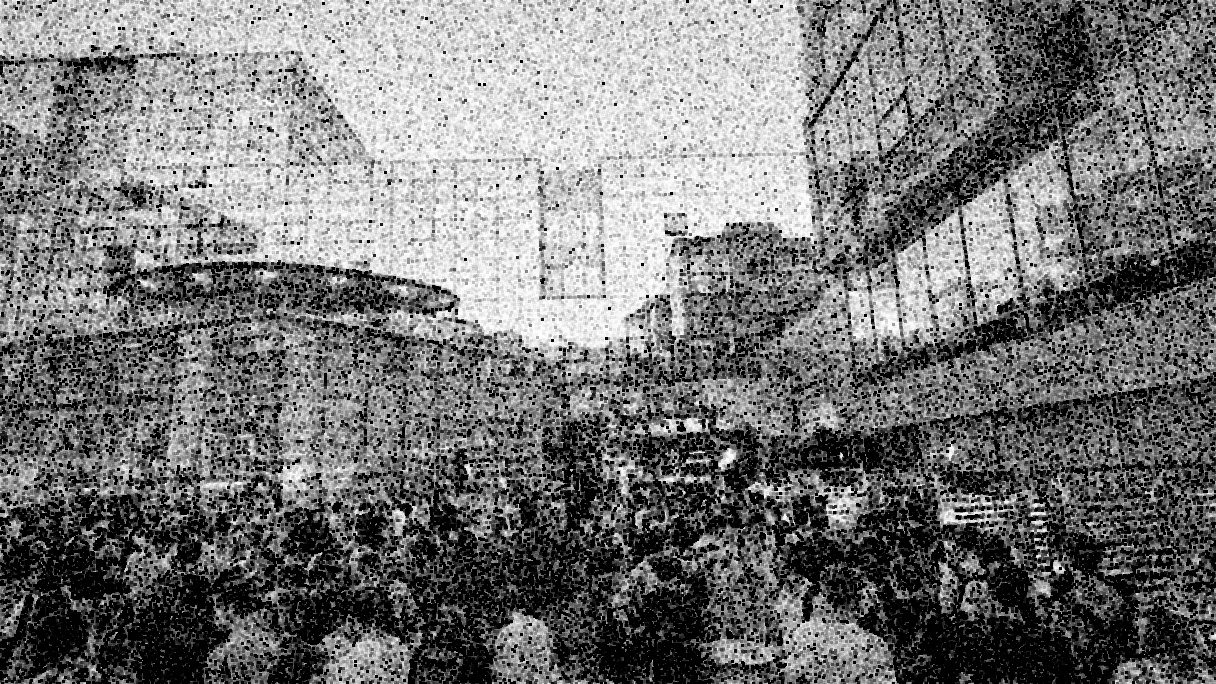
\includegraphics[width=\textwidth]{images/2_low_filters/gaussian - contrharmonic (Q=-1.5).jpg}
        \caption{Гауссов шум + фильтр ($Q = -1.5$)}
    \end{minipage}\hfill
    \begin{minipage}{0.49\textwidth}
        \centering 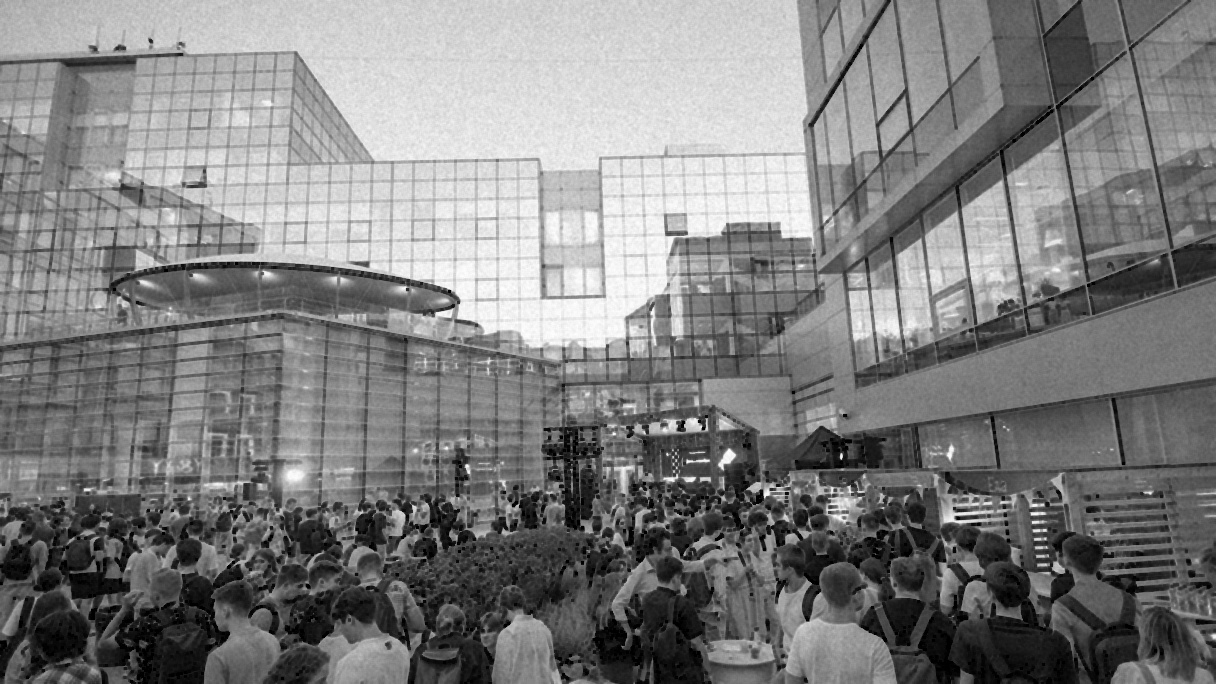
\includegraphics[width=\textwidth]{images/2_low_filters/poisson - contrharmonic (Q=-1.5).jpg}
        \caption{Шум квантования + фильтр ($Q = -1.5$)}
    \end{minipage}
\end{figure}
\begin{figure}[H]
    \begin{minipage}{0.49\textwidth}
        \centering 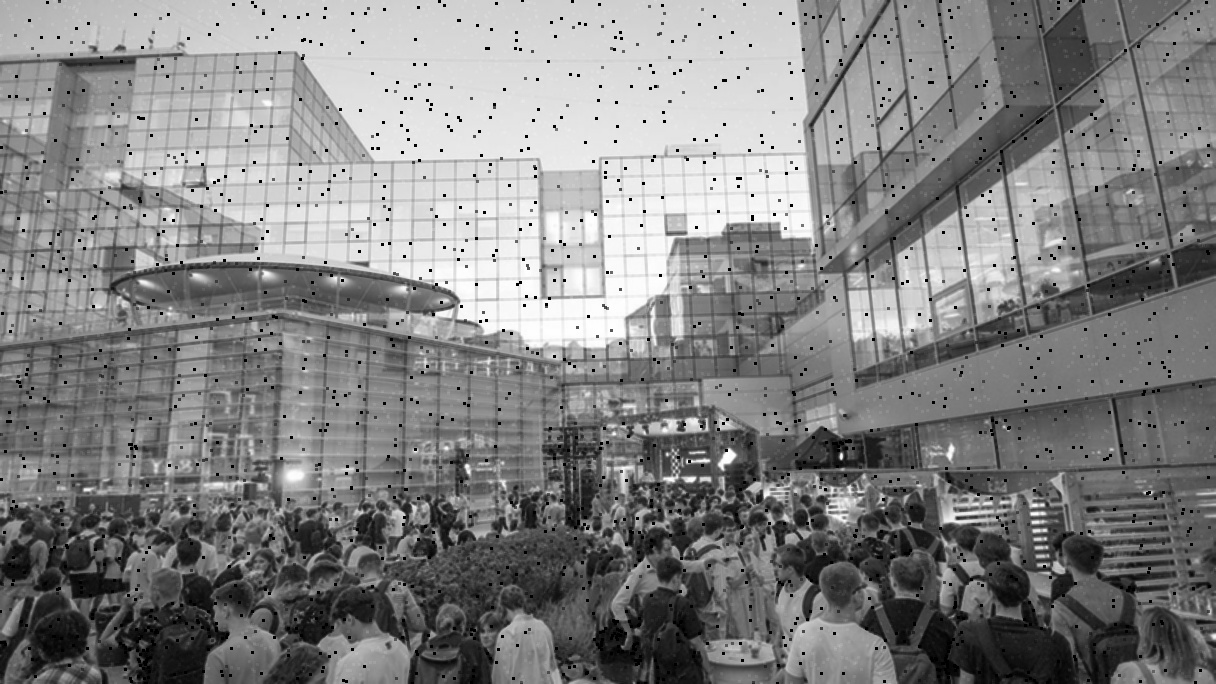
\includegraphics[width=\textwidth]{images/2_low_filters/impulse - contrharmonic (Q=-0.5).jpg}
        \caption{Импульсный шум + фильтр ($Q = -0.5$)}
    \end{minipage}\hfill
    \begin{minipage}{0.49\textwidth}
        \centering 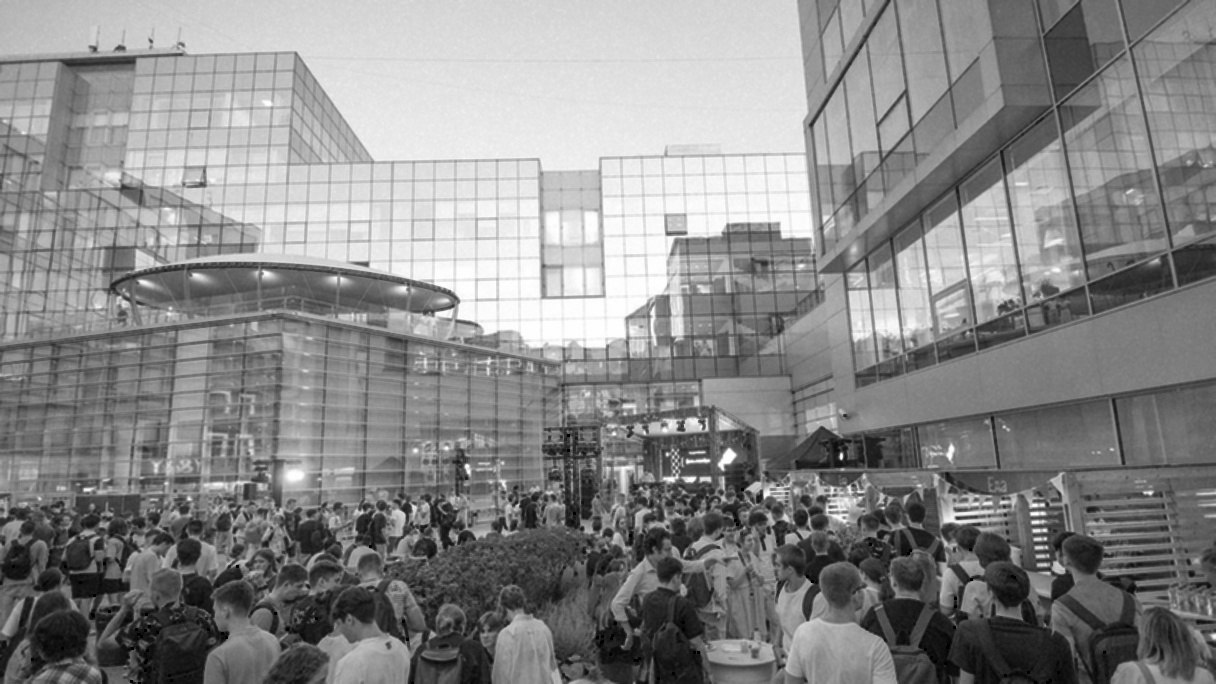
\includegraphics[width=\textwidth]{images/2_low_filters/additive - contrharmonic (Q=-0.5).jpg}
        \caption{Аддитивный шум + фильтр ($Q = -0.5$)}
    \end{minipage}
\end{figure}
\begin{figure}[H]
    \begin{minipage}{0.49\textwidth}
        \centering 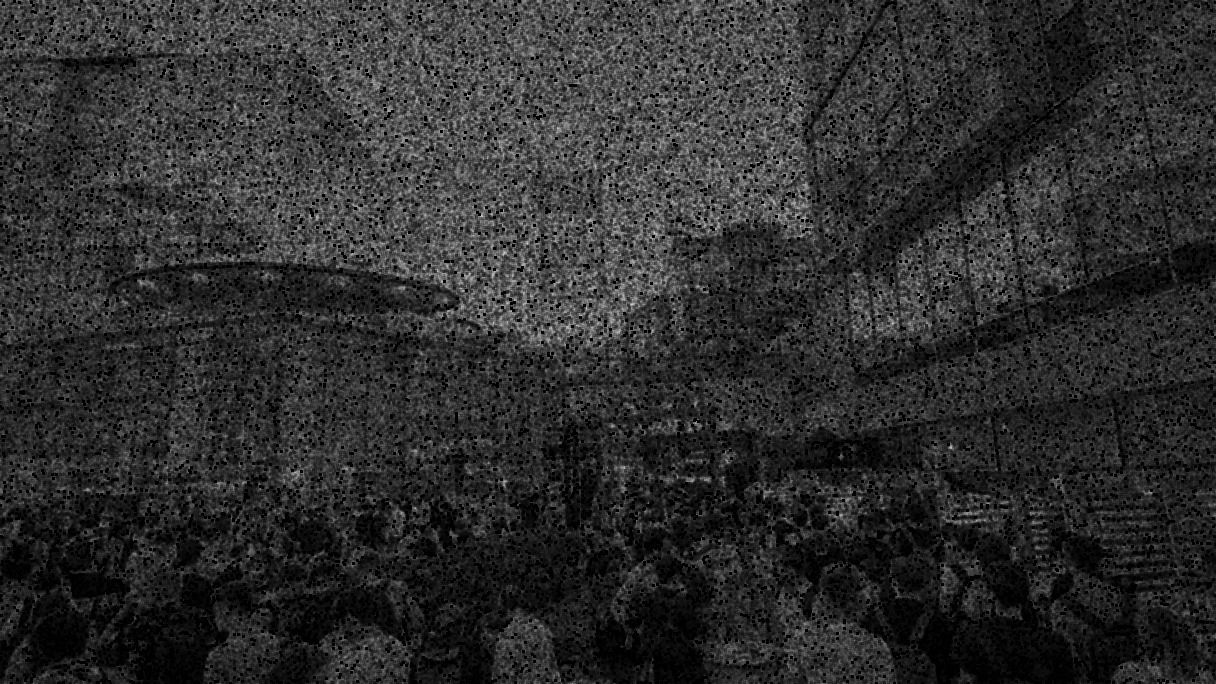
\includegraphics[width=\textwidth]{images/2_low_filters/multiplicative - contrharmonic (Q=-0.5).jpg}
        \caption{Мульти-ный шум + фильтр ($Q = -0.5$)}
    \end{minipage}\hfill
    \begin{minipage}{0.49\textwidth}
        \centering 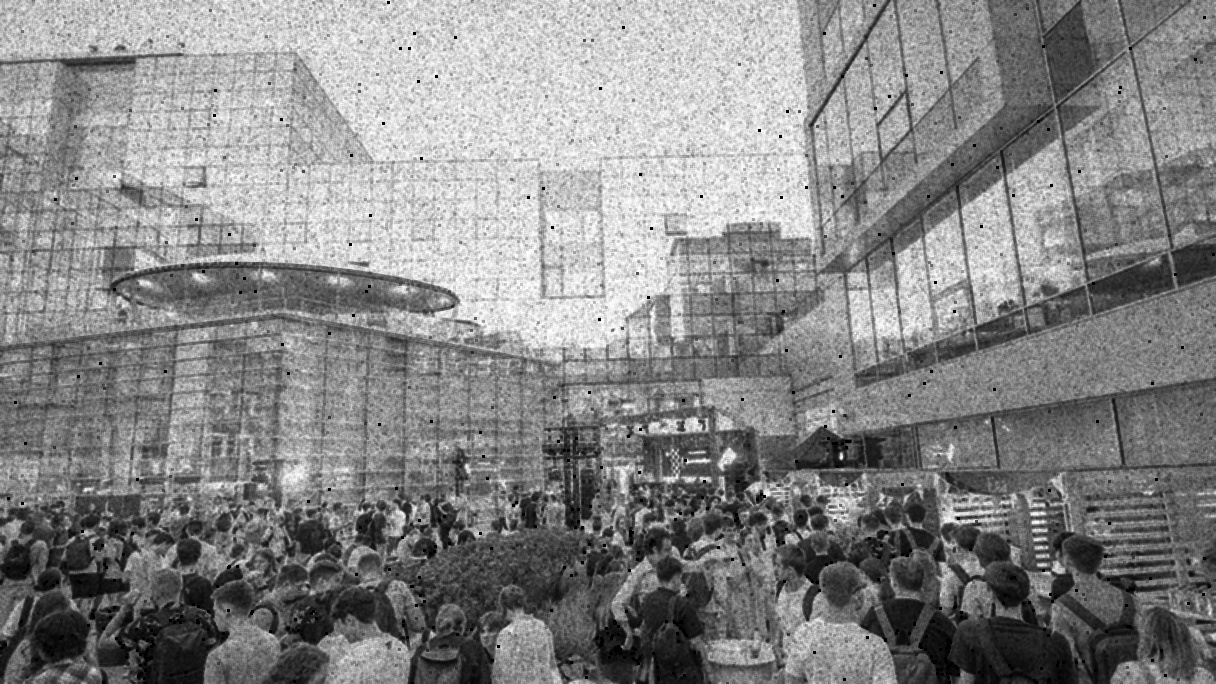
\includegraphics[width=\textwidth]{images/2_low_filters/speckle - contrharmonic (Q=-0.5).jpg}
        \caption{Спекл-шум + фильтр ($Q = -0.5$)}
    \end{minipage}
\end{figure}
\begin{figure}[H]
    \begin{minipage}{0.49\textwidth}
        \centering 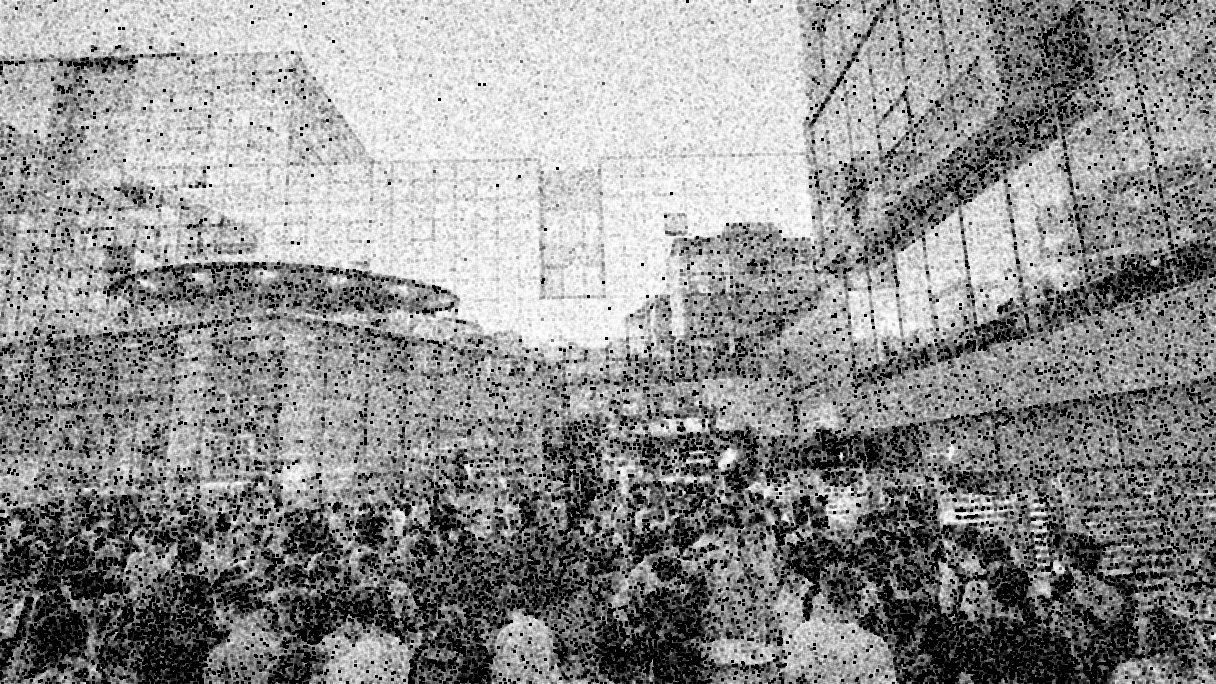
\includegraphics[width=\textwidth]{images/2_low_filters/gaussian - contrharmonic (Q=-0.5).jpg}
        \caption{Гауссов шум + фильтр ($Q = -0.5$)}
    \end{minipage}\hfill
    \begin{minipage}{0.49\textwidth}
        \centering 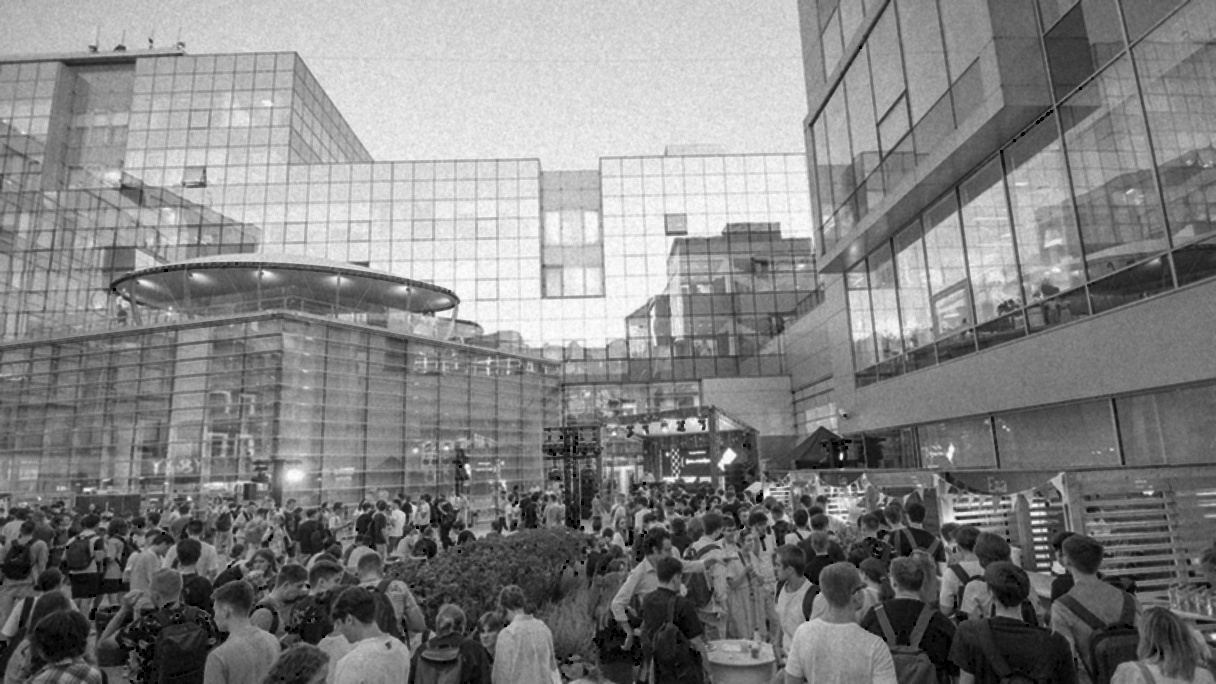
\includegraphics[width=\textwidth]{images/2_low_filters/poisson - contrharmonic (Q=-0.5).jpg}
        \caption{Шум квантования + фильтр ($Q = -0.5$)}
    \end{minipage}
\end{figure}
\begin{figure}[H]
    \begin{minipage}{0.49\textwidth}
        \centering 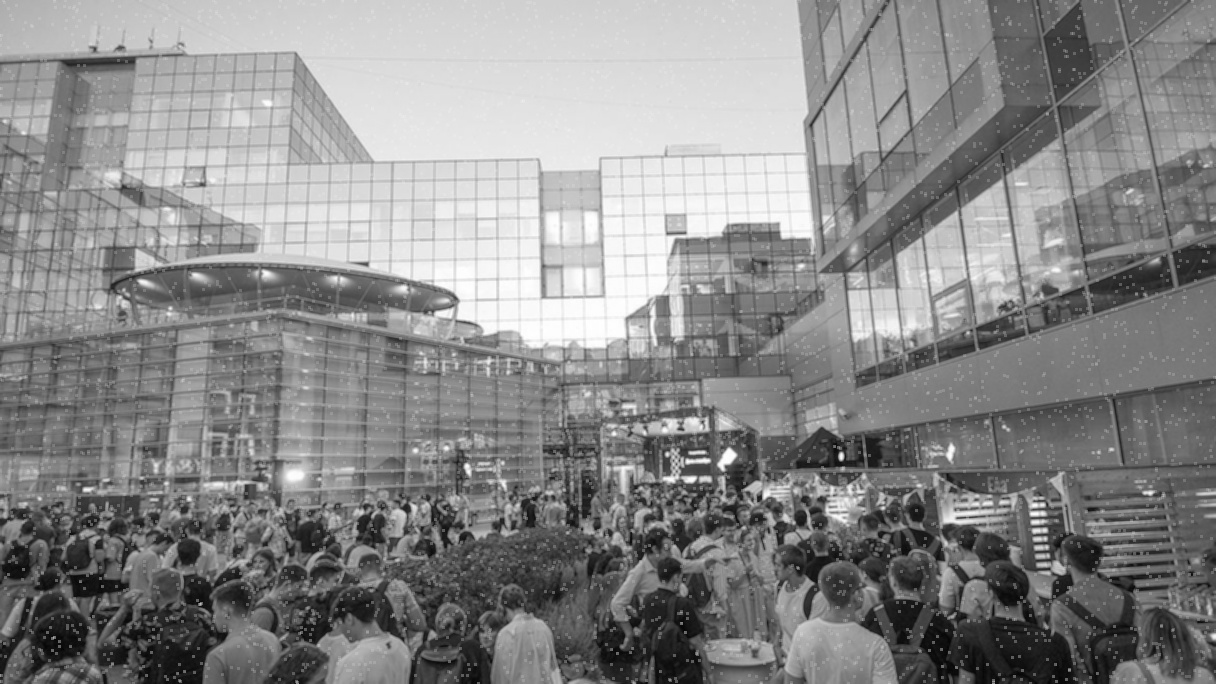
\includegraphics[width=\textwidth]{images/2_low_filters/impulse - contrharmonic (Q=0.5).jpg}
        \caption{Импульсный шум + фильтр ($Q = 0.5$)}
    \end{minipage}\hfill
    \begin{minipage}{0.49\textwidth}
        \centering 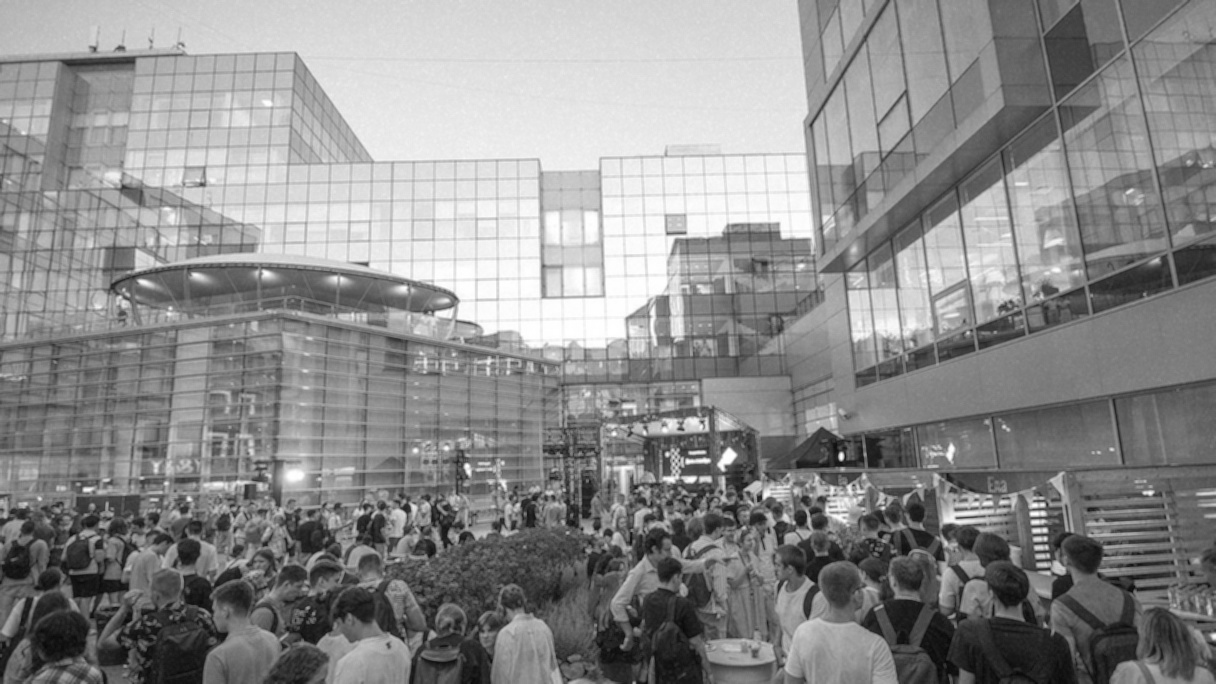
\includegraphics[width=\textwidth]{images/2_low_filters/additive - contrharmonic (Q=0.5).jpg}
        \caption{Аддитивный шум + фильтр ($Q = 0.5$)}
    \end{minipage}
\end{figure}
\begin{figure}[H]
    \begin{minipage}{0.49\textwidth}
        \centering 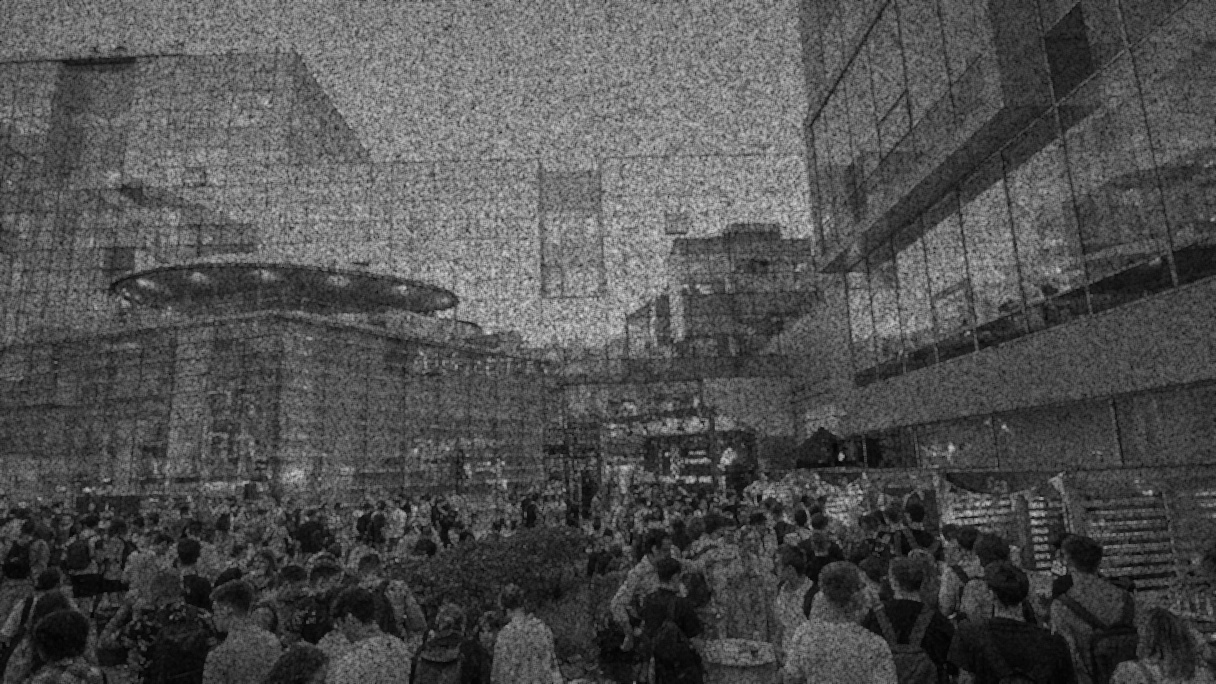
\includegraphics[width=\textwidth]{images/2_low_filters/multiplicative - contrharmonic (Q=0.5).jpg}
        \caption{Мульти-ный шум + фильтр ($Q = 0.5$)}
    \end{minipage}\hfill
    \begin{minipage}{0.49\textwidth}
        \centering 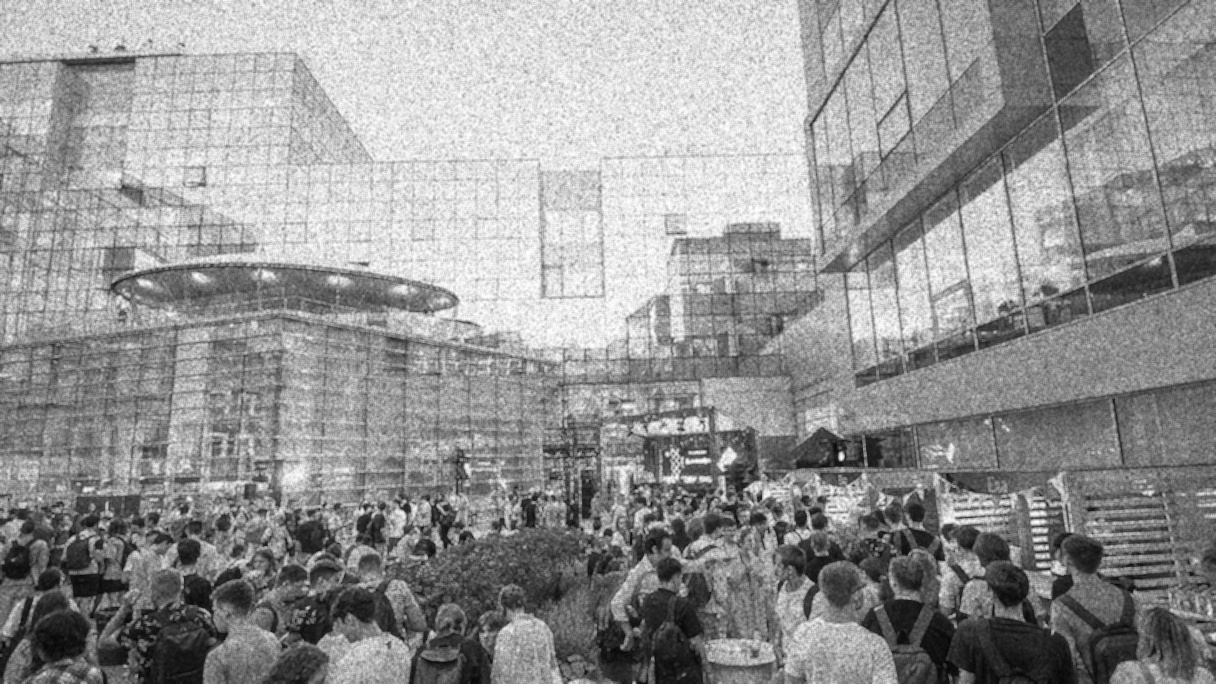
\includegraphics[width=\textwidth]{images/2_low_filters/speckle - contrharmonic (Q=0.5).jpg}
        \caption{Спекл-шум + фильтр ($Q = 0.5$)}
    \end{minipage}
\end{figure}
\begin{figure}[H]
    \begin{minipage}{0.49\textwidth}
        \centering 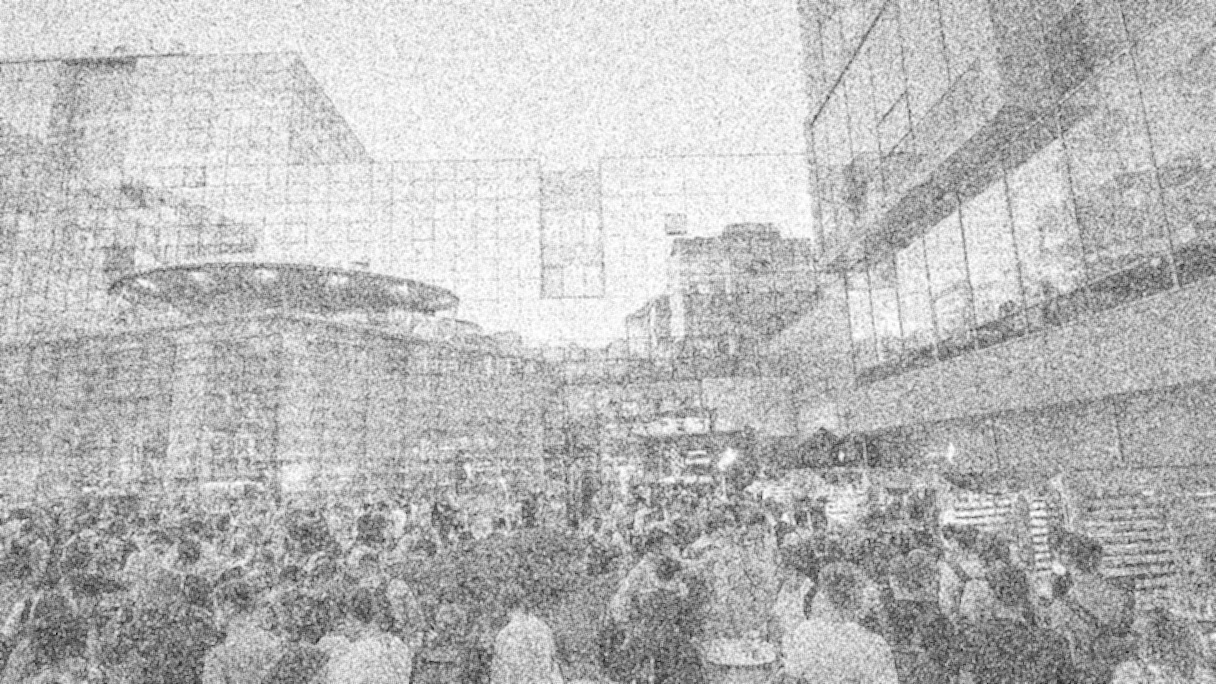
\includegraphics[width=\textwidth]{images/2_low_filters/gaussian - contrharmonic (Q=0.5).jpg}
        \caption{Гауссов шум + фильтр ($Q = 0.5$)}
    \end{minipage}\hfill
    \begin{minipage}{0.49\textwidth}
        \centering 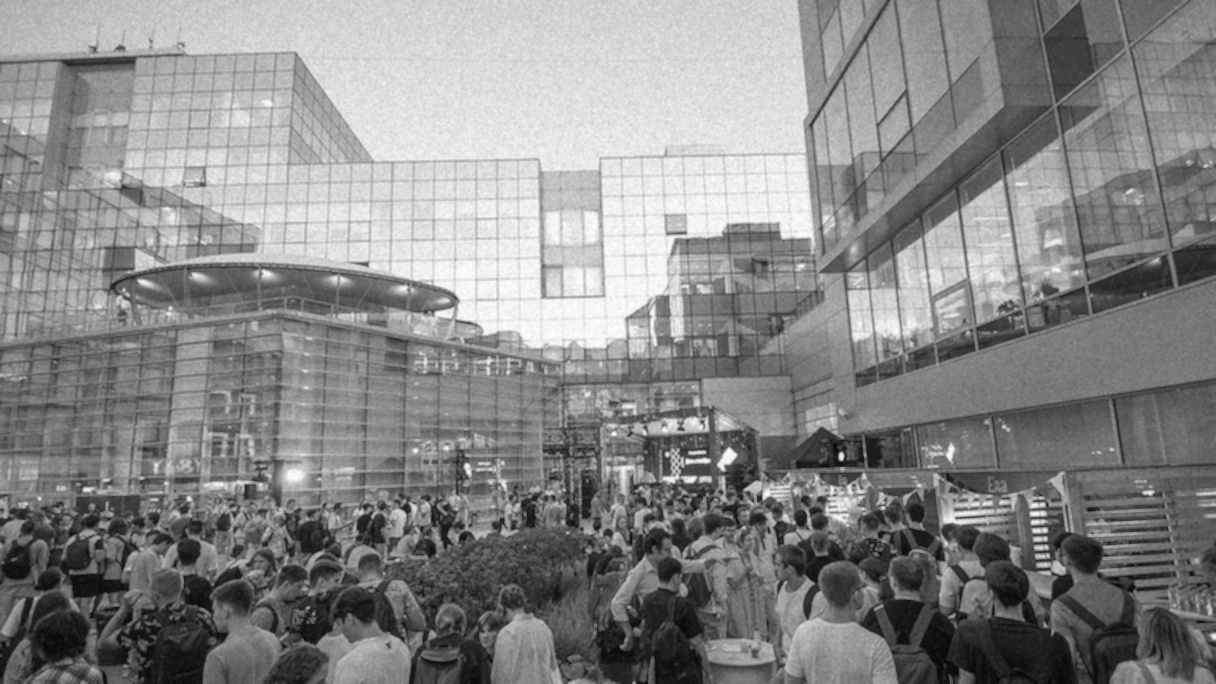
\includegraphics[width=\textwidth]{images/2_low_filters/poisson - contrharmonic (Q=0.5).jpg}
        \caption{Шум квантования + фильтр ($Q = 0.5$)}
    \end{minipage}
\end{figure}
\begin{figure}[H]
    \begin{minipage}{0.49\textwidth}
        \centering 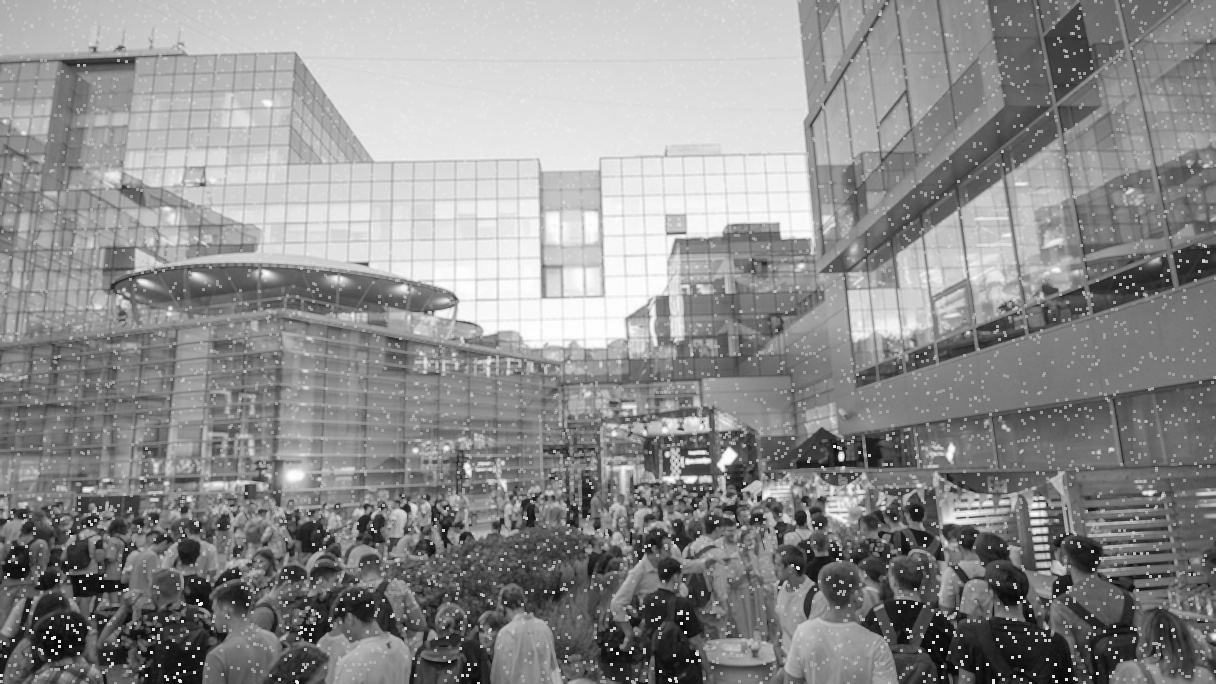
\includegraphics[width=\textwidth]{images/2_low_filters/impulse - contrharmonic (Q=1.5).jpg}
        \caption{Импульсный шум + фильтр ($Q = 1.5$)}
    \end{minipage}\hfill
    \begin{minipage}{0.49\textwidth}
        \centering 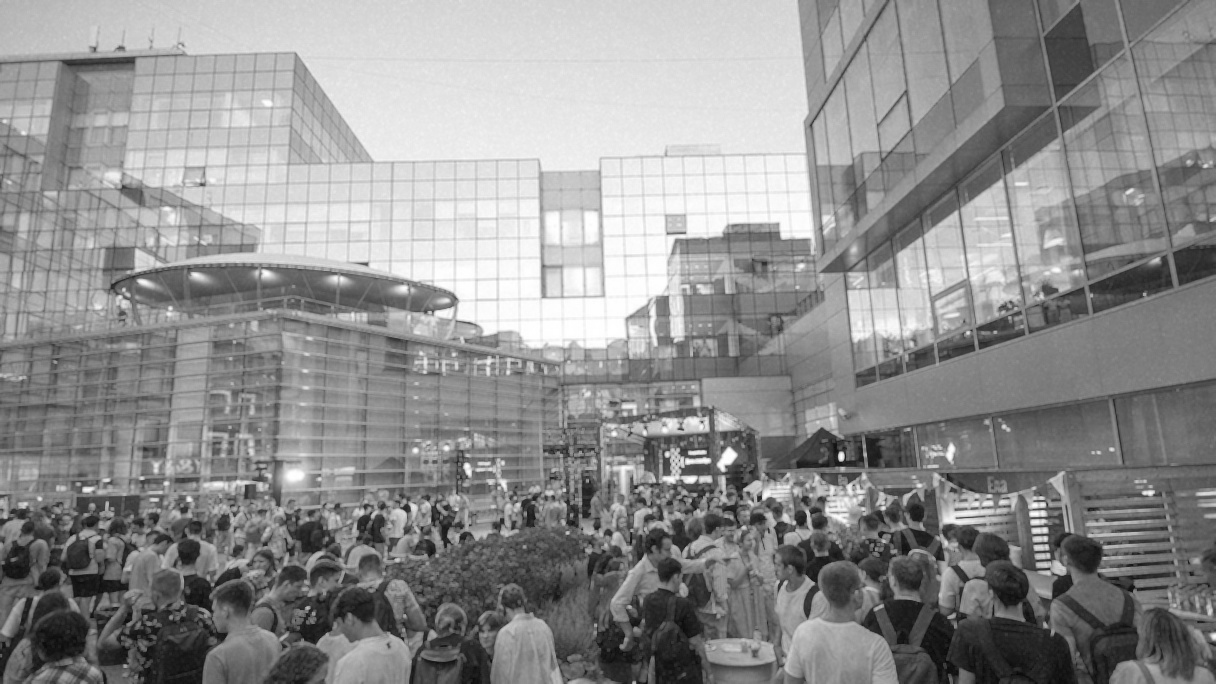
\includegraphics[width=\textwidth]{images/2_low_filters/additive - contrharmonic (Q=1.5).jpg}
        \caption{Аддитивный шум + фильтр ($Q = 1.5$)}
    \end{minipage}
\end{figure}
\begin{figure}[H]
    \begin{minipage}{0.49\textwidth}
        \centering 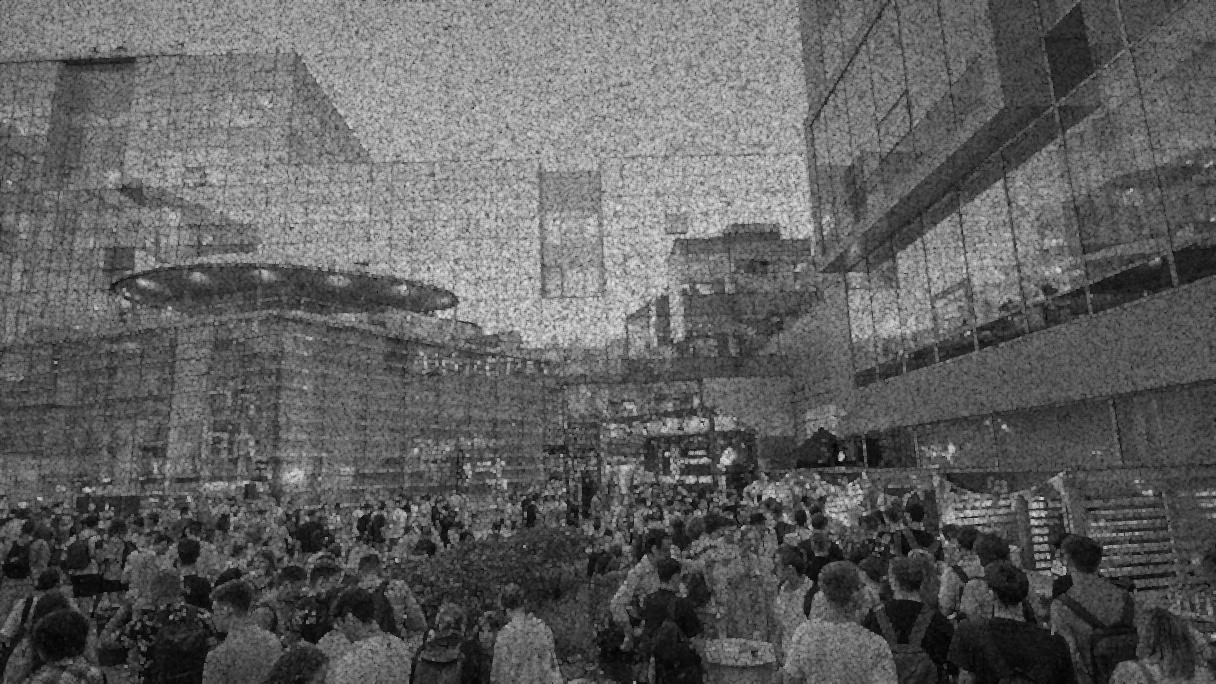
\includegraphics[width=\textwidth]{images/2_low_filters/multiplicative - contrharmonic (Q=1.5).jpg}
        \caption{Мульти-ный шум + фильтр ($Q = 1.5$)}
    \end{minipage}\hfill
    \begin{minipage}{0.49\textwidth}
        \centering 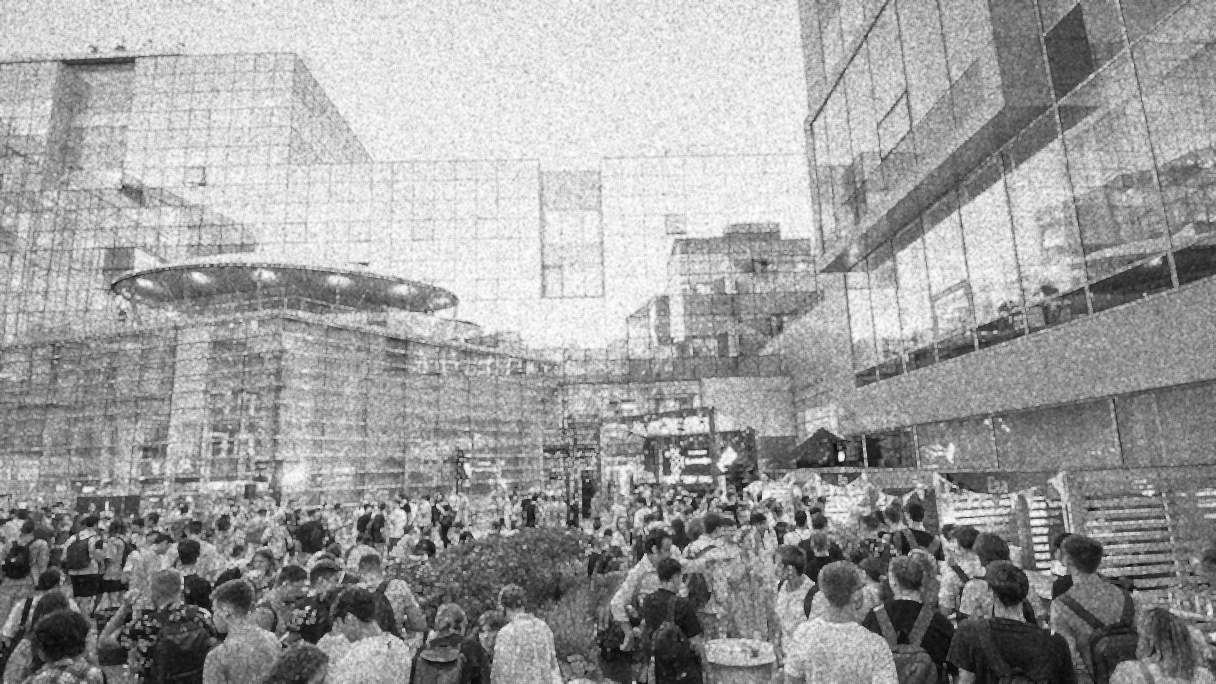
\includegraphics[width=\textwidth]{images/2_low_filters/speckle - contrharmonic (Q=1.5).jpg}
        \caption{Спекл-шум + фильтр ($Q = 1.5$)}
    \end{minipage}
\end{figure}
\begin{figure}[H]
    \begin{minipage}{0.49\textwidth}
        \centering 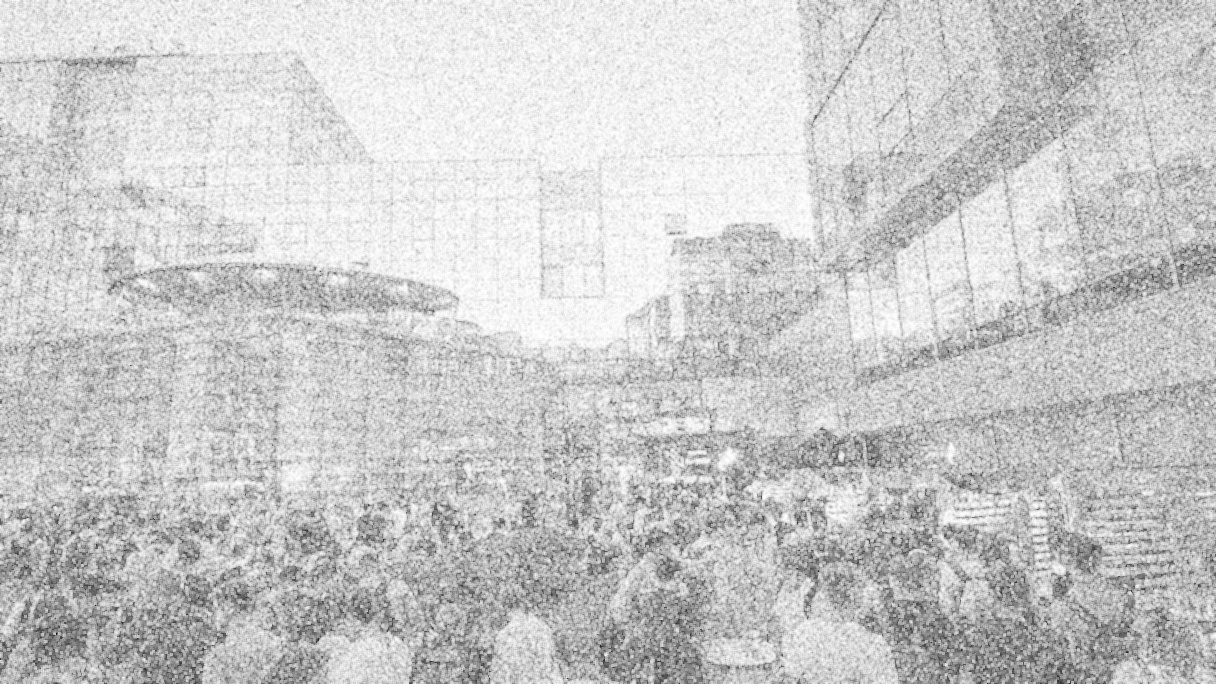
\includegraphics[width=\textwidth]{images/2_low_filters/gaussian - contrharmonic (Q=1.5).jpg}
        \caption{Гауссов шум + фильтр ($Q = 1.5$)}
    \end{minipage}\hfill
    \begin{minipage}{0.49\textwidth}
        \centering 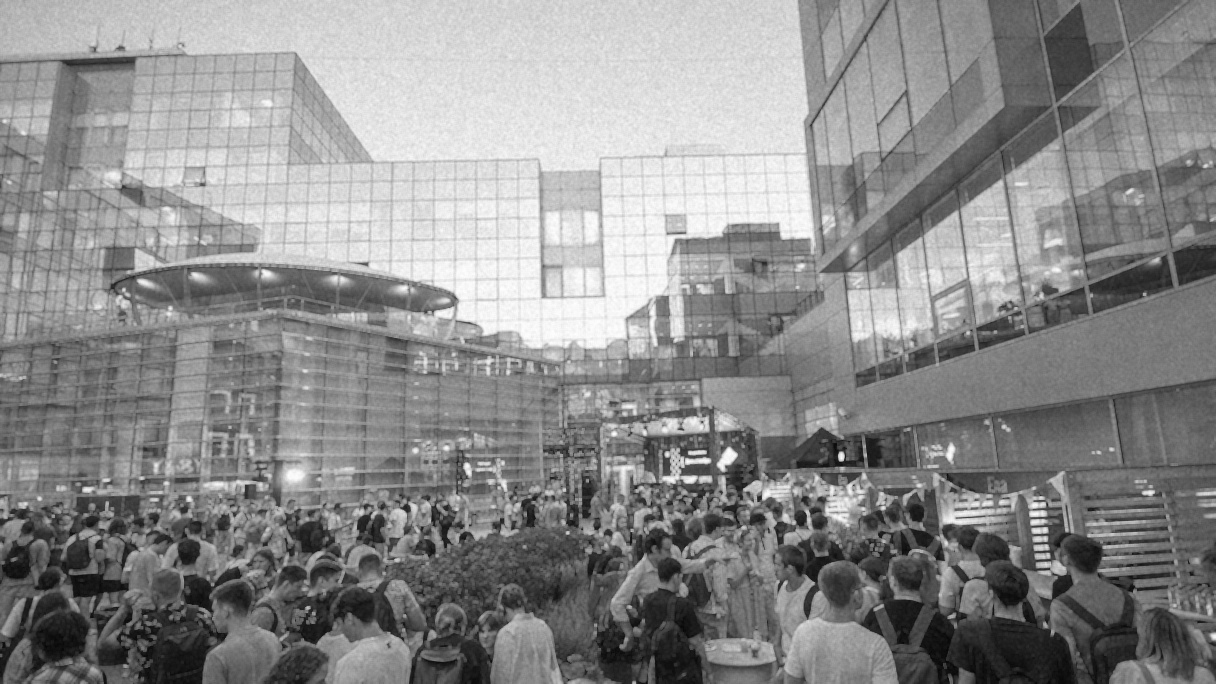
\includegraphics[width=\textwidth]{images/2_low_filters/poisson - contrharmonic (Q=1.5).jpg}
        \caption{Шум квантования + фильтр ($Q = 1.5$)}
    \end{minipage}
\end{figure}
\noindent Работу контргармонического усредняющего фильтра хорошо видно на импульсном шуме. Действительно, на отрицательных значениях $Q$ мы видим чёрные точки и при этом белые подавляются, а при положительных значениях $Q$ всё наоборот. Но с аддитивным шумом фильтр работает плохо --- тёмные или светлые контуры (в зависимости от знака $Q$) размываются. \pagebreak

% MARK: Нелинейные фильтры
\addsection{Нелинейная фильтрация (покупайте нелинейки, чтобы разобраться)}
Низкочастотные фильтры хороши, когда шум основан на нормальном распределении --- они сглаживают изображение, оставляя только высокочастотные компоненты, но это не самый оптимальный метод. Ведь существуют нелинейные фильтры, которые могут устранять импульсные помехи другими способами.
% MARK: Медианный фильтр
\addsubsection{Медианный фильтр}
И начнём с одного из главного нелинейного фильтра --- обыкновенного медианного фильтра. Среди пикселей, попавших в окно фильтрации, выбирается медианный по интенсивности. Посмотрим на результат работы фильтра, применённого к зашумленным разными методами изображениям, с разными размерами окон:
\begin{figure}[H]
    \begin{minipage}{0.49\textwidth}
        \centering 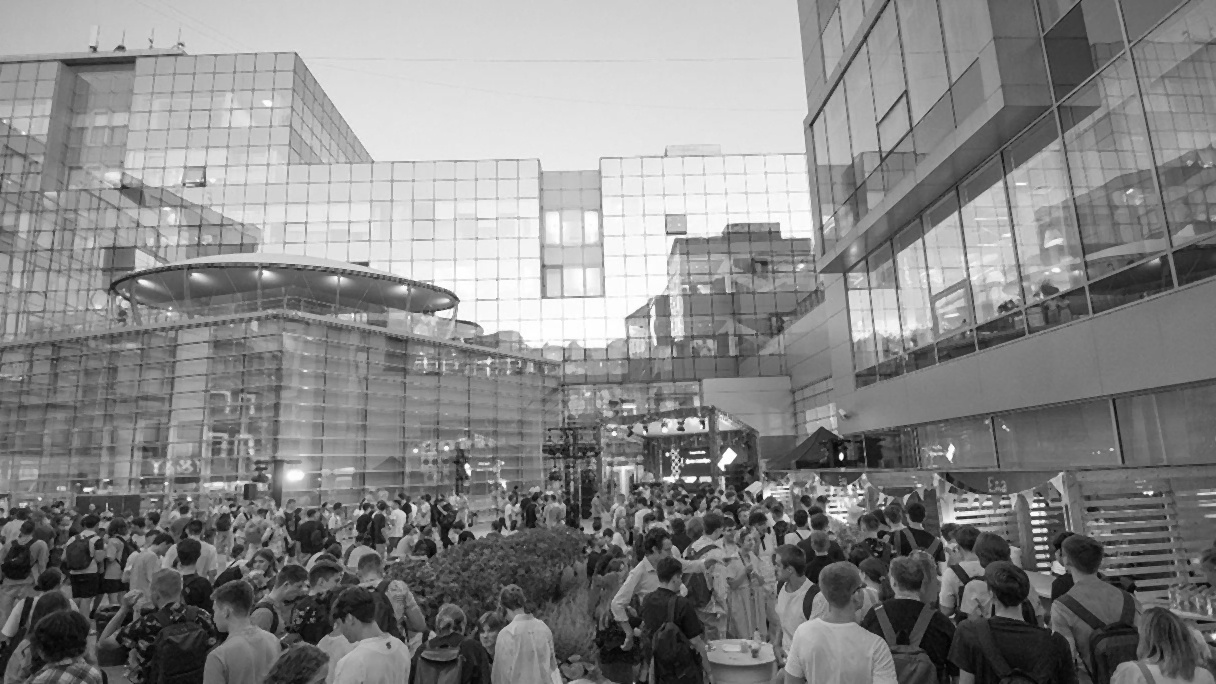
\includegraphics[width=\textwidth]{images/3_nonlinear_filters/impulse - median (ksize=3).jpg}
        \caption{Импульсный шум + фильтр ($ksize = 3$)}
    \end{minipage}\hfill
    \begin{minipage}{0.49\textwidth}
        \centering 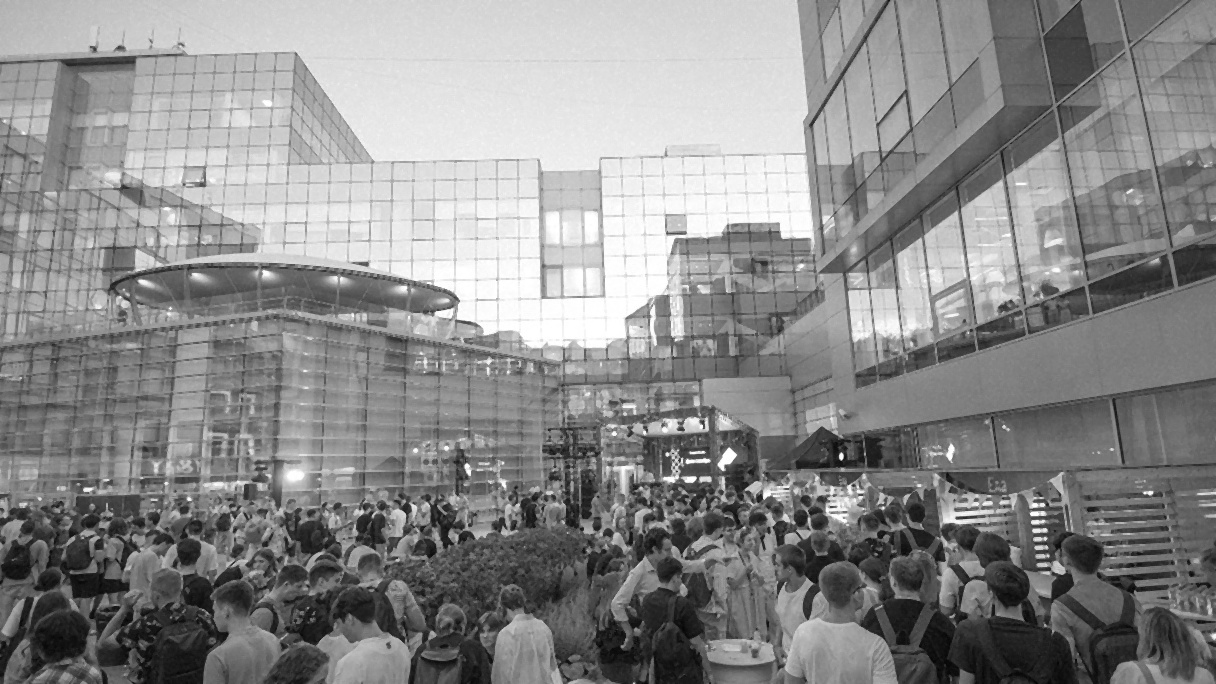
\includegraphics[width=\textwidth]{images/3_nonlinear_filters/additive - median (ksize=3).jpg}
        \caption{Аддитивный шум + фильтр ($ksize = 3$)}
    \end{minipage}
\end{figure}
\begin{figure}[H]
    \begin{minipage}{0.49\textwidth}
        \centering 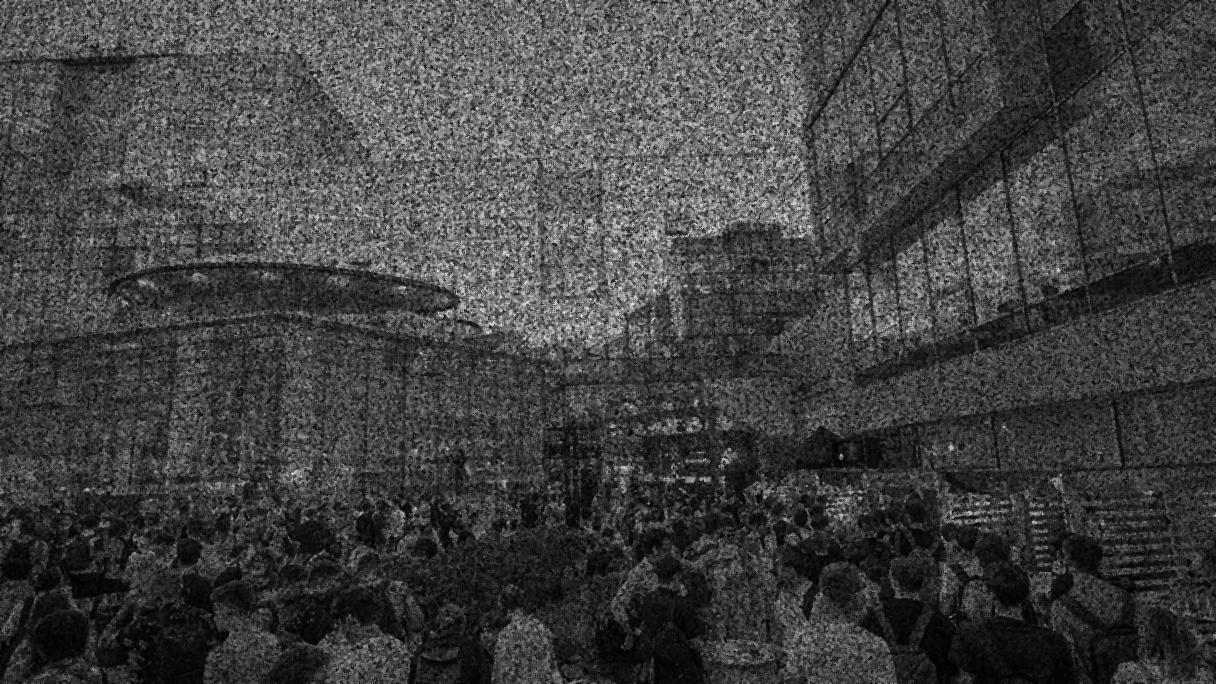
\includegraphics[width=\textwidth]{images/3_nonlinear_filters/multiplicative - median (ksize=3).jpg}
        \caption{Мульти-ный шум + фильтр ($ksize = 3$)}
    \end{minipage}\hfill
    \begin{minipage}{0.49\textwidth}
        \centering 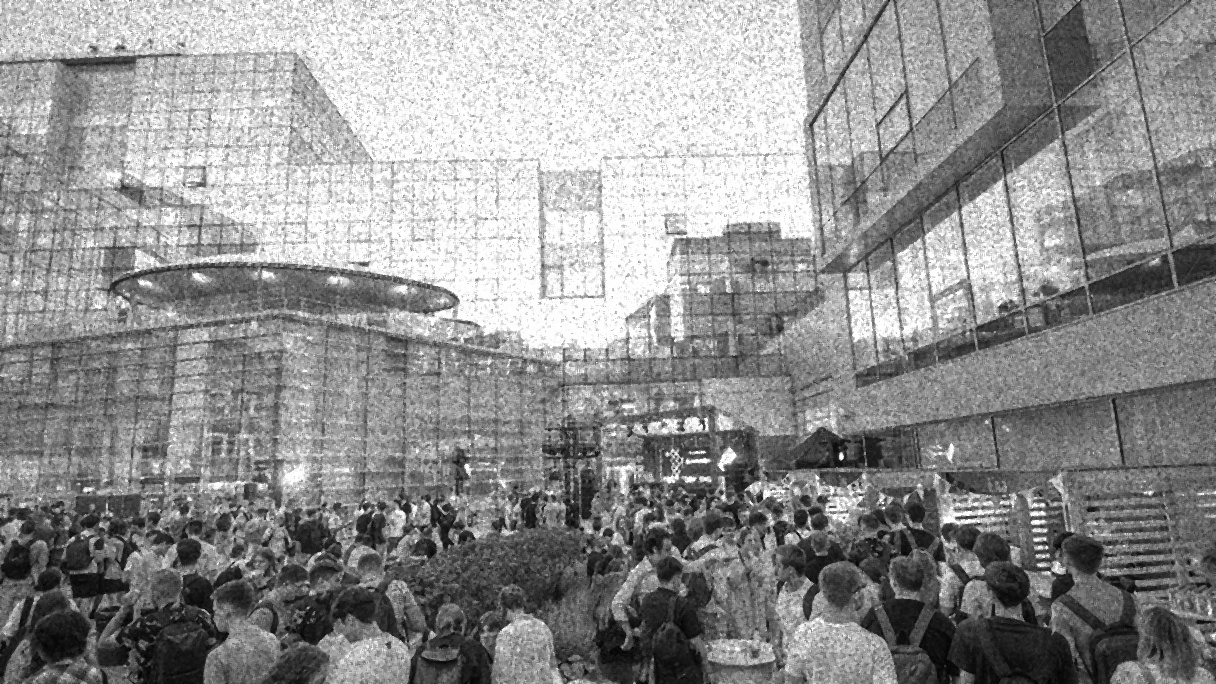
\includegraphics[width=\textwidth]{images/3_nonlinear_filters/speckle - median (ksize=3).jpg}
        \caption{Спекл-шум + фильтр ($ksize = 3$)}
    \end{minipage}
\end{figure}
\begin{figure}[H]
    \begin{minipage}{0.49\textwidth}
        \centering 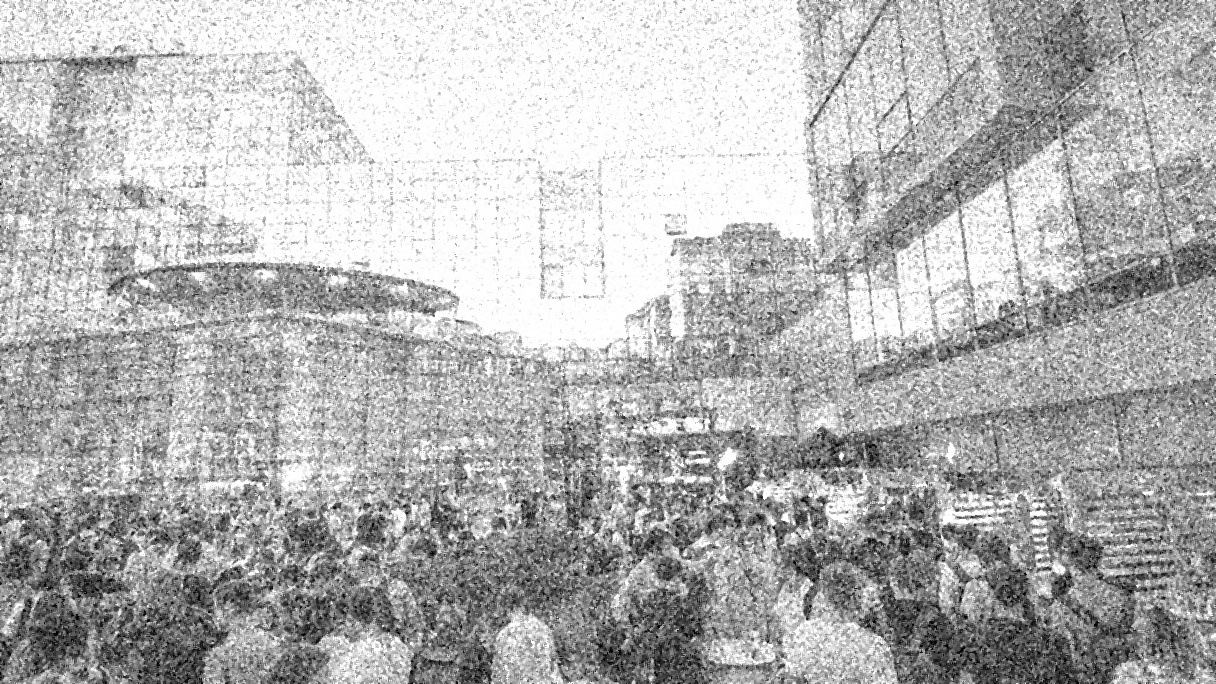
\includegraphics[width=\textwidth]{images/3_nonlinear_filters/gaussian - median (ksize=3).jpg}
        \caption{Гауссов шум + фильтр ($ksize = 3$)}
    \end{minipage}\hfill
    \begin{minipage}{0.49\textwidth}
        \centering 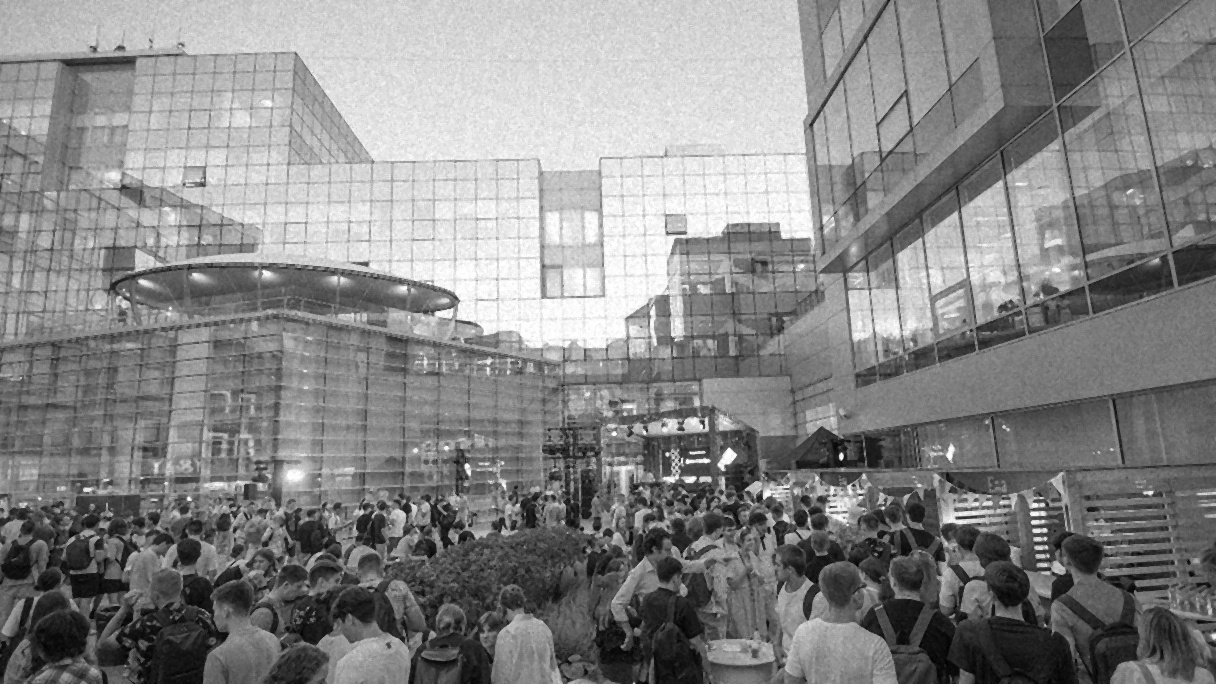
\includegraphics[width=\textwidth]{images/3_nonlinear_filters/poisson - median (ksize=3).jpg}
        \caption{Шум квантования + фильтр ($ksize = 3$)}
    \end{minipage}
\end{figure}
\begin{figure}[H]
    \begin{minipage}{0.49\textwidth}
        \centering 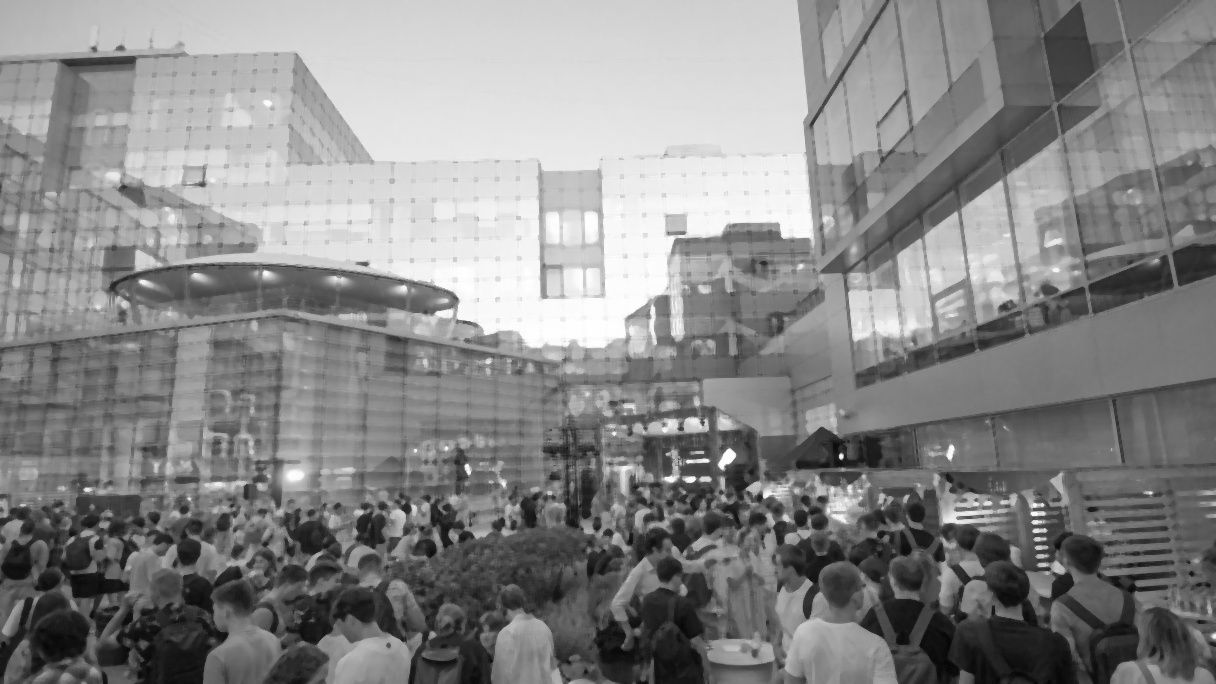
\includegraphics[width=\textwidth]{images/3_nonlinear_filters/impulse - median (ksize=5).jpg}
        \caption{Импульсный шум + фильтр ($ksize = 5$)}
    \end{minipage}\hfill
    \begin{minipage}{0.49\textwidth}
        \centering 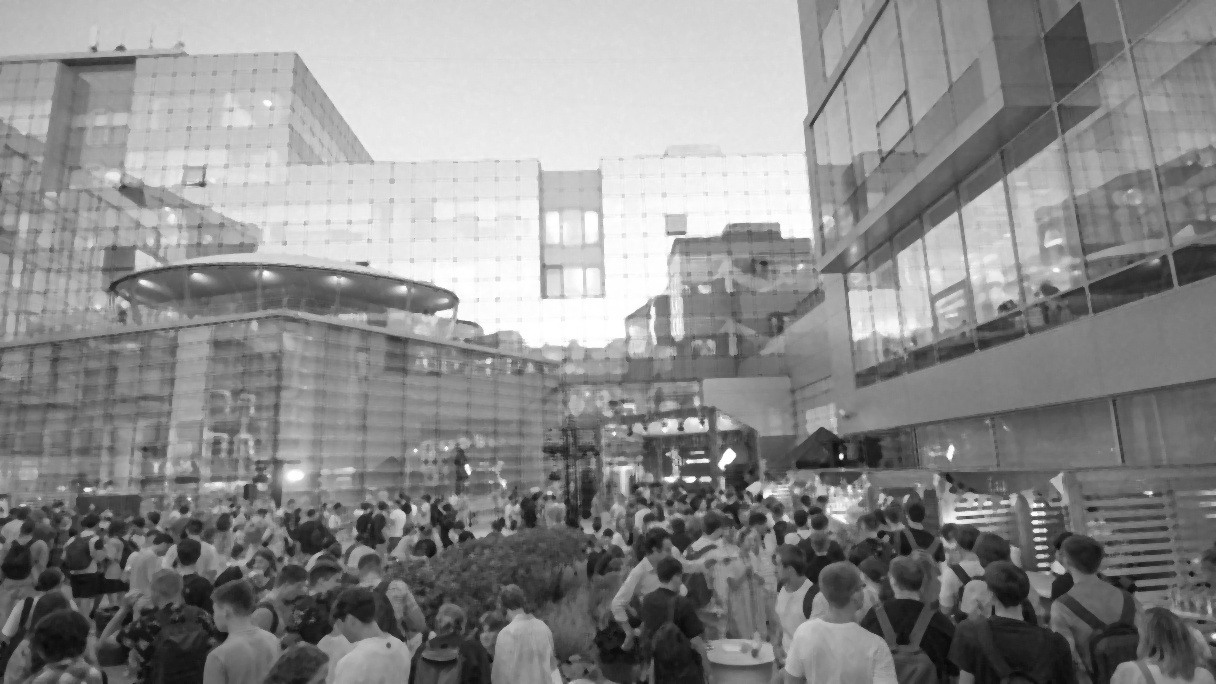
\includegraphics[width=\textwidth]{images/3_nonlinear_filters/additive - median (ksize=5).jpg}
        \caption{Аддитивный шум + фильтр ($ksize = 5$)}
    \end{minipage}
\end{figure}
\begin{figure}[H]
    \begin{minipage}{0.49\textwidth}
        \centering 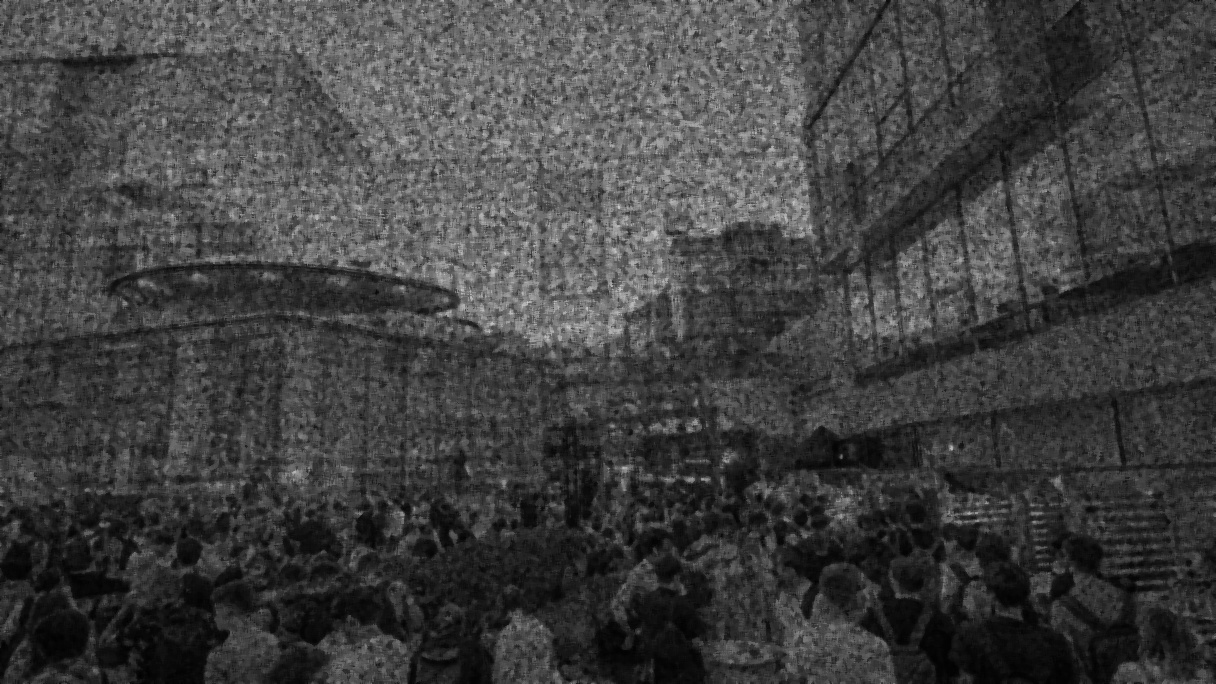
\includegraphics[width=\textwidth]{images/3_nonlinear_filters/multiplicative - median (ksize=5).jpg}
        \caption{Мульти-ный шум + фильтр ($ksize = 5$)}
    \end{minipage}\hfill
    \begin{minipage}{0.49\textwidth}
        \centering 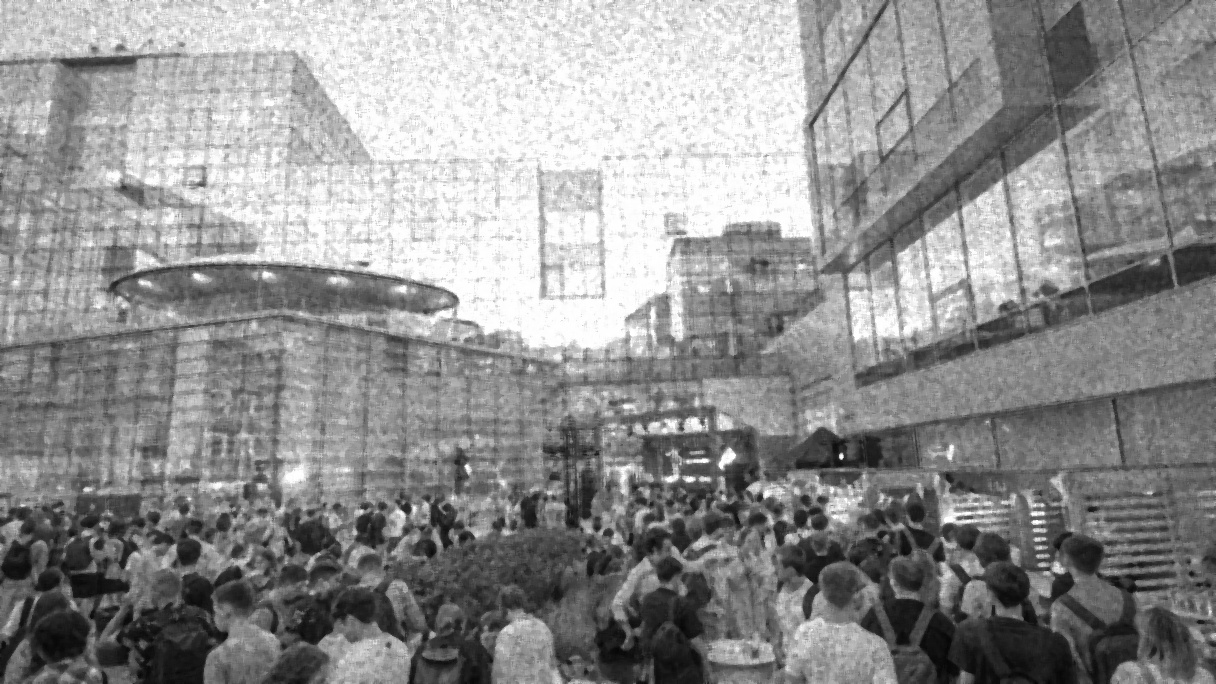
\includegraphics[width=\textwidth]{images/3_nonlinear_filters/speckle - median (ksize=5).jpg}
        \caption{Спекл-шум + фильтр ($ksize = 5$)}
    \end{minipage}
\end{figure}
\begin{figure}[H]
    \begin{minipage}{0.49\textwidth}
        \centering 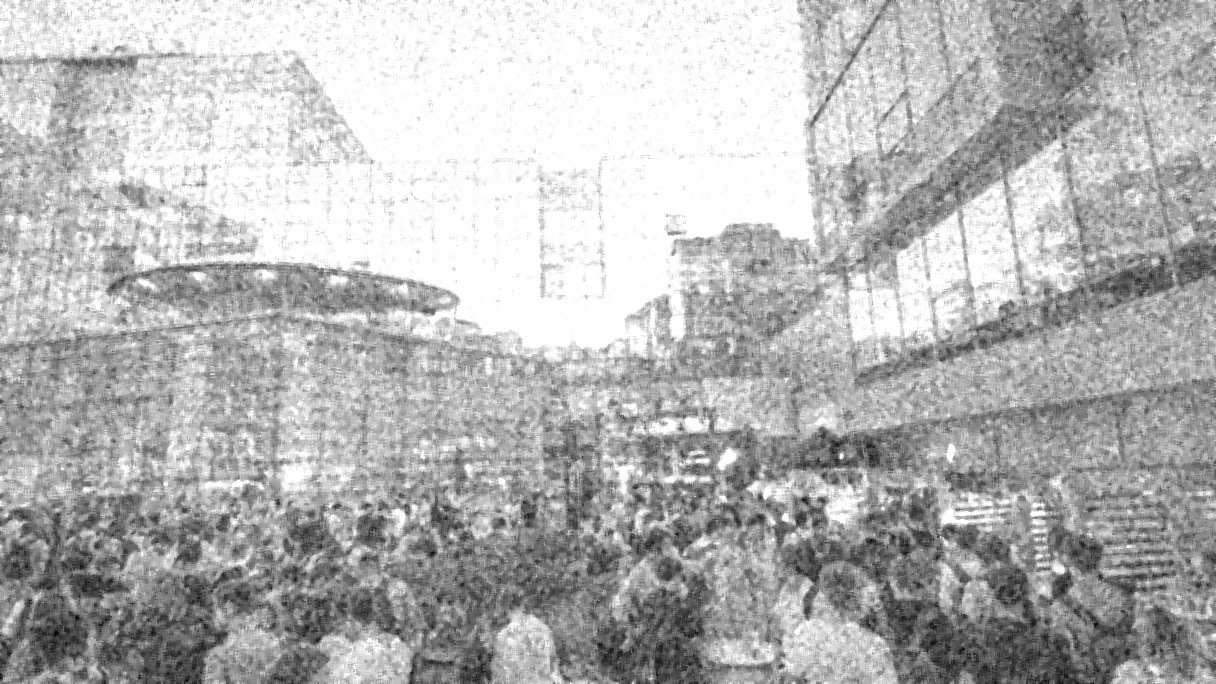
\includegraphics[width=\textwidth]{images/3_nonlinear_filters/gaussian - median (ksize=5).jpg}
        \caption{Гауссов шум + фильтр ($ksize = 5$)}
    \end{minipage}\hfill
    \begin{minipage}{0.49\textwidth}
        \centering 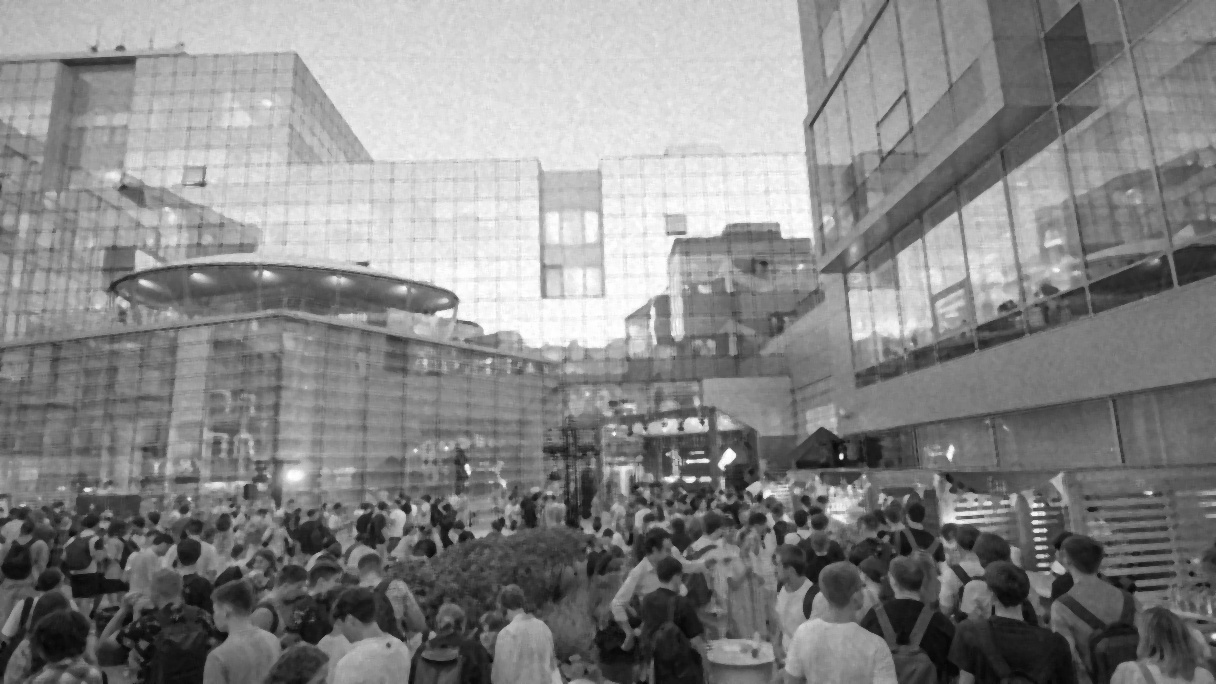
\includegraphics[width=\textwidth]{images/3_nonlinear_filters/poisson - median (ksize=5).jpg}
        \caption{Шум квантования + фильтр ($ksize = 5$)}
    \end{minipage}
\end{figure}
\begin{figure}[H]
    \begin{minipage}{0.49\textwidth}
        \centering 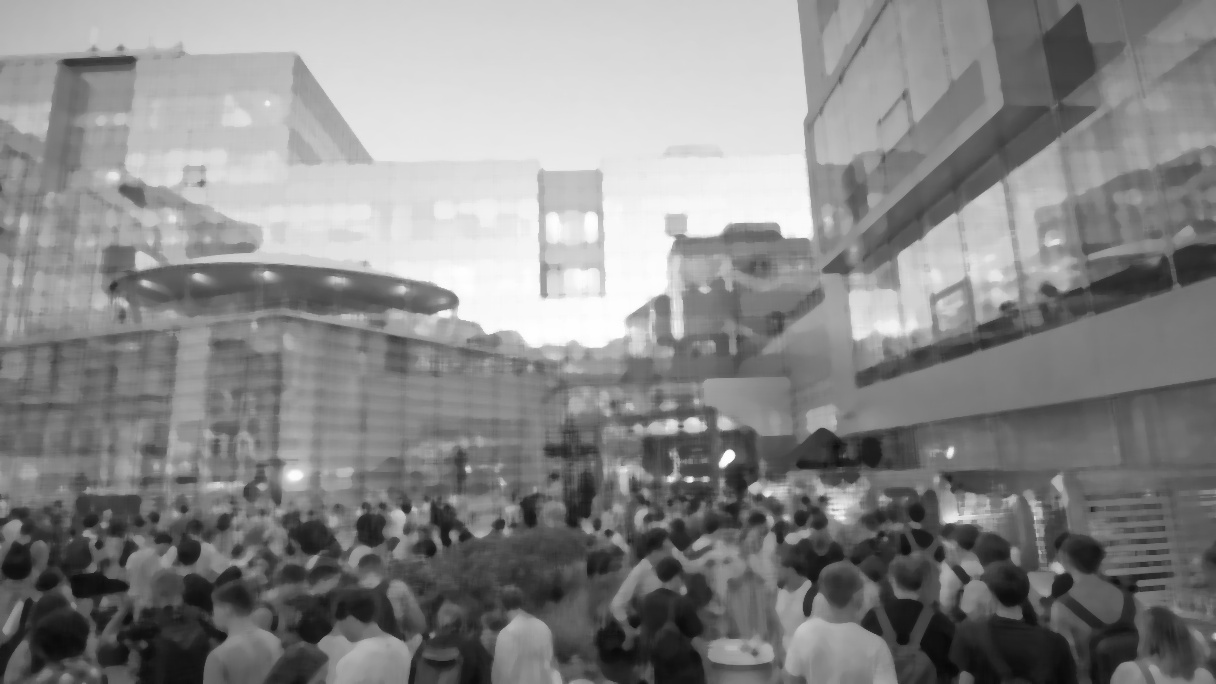
\includegraphics[width=\textwidth]{images/3_nonlinear_filters/impulse - median (ksize=9).jpg}
        \caption{Импульсный шум + фильтр ($ksize = 9$)}
    \end{minipage}\hfill
    \begin{minipage}{0.49\textwidth}
        \centering \includegraphics[width=\textwidth]{images/3_nonlinear_filters/additive - median (ksize=9).jpg}
        \caption{Аддитивный шум + фильтр ($ksize = 9$)}
    \end{minipage}
\end{figure}
\begin{figure}[H]
    \begin{minipage}{0.49\textwidth}
        \centering \includegraphics[width=\textwidth]{images/3_nonlinear_filters/multiplicative - median (ksize=9).jpg}
        \caption{Мульти-ный шум + фильтр ($ksize = 9$)}
    \end{minipage}\hfill
    \begin{minipage}{0.49\textwidth}
        \centering \includegraphics[width=\textwidth]{images/3_nonlinear_filters/speckle - median (ksize=9).jpg}
        \caption{Спекл-шум + фильтр ($ksize = 9$)}
    \end{minipage}
\end{figure}
\begin{figure}[H]
    \begin{minipage}{0.49\textwidth}
        \centering \includegraphics[width=\textwidth]{images/3_nonlinear_filters/gaussian - median (ksize=9).jpg}
        \caption{Гауссов шум + фильтр ($ksize = 9$)}
    \end{minipage}\hfill
    \begin{minipage}{0.49\textwidth}
        \centering \includegraphics[width=\textwidth]{images/3_nonlinear_filters/poisson - median (ksize=9).jpg}
        \caption{Шум квантования + фильтр ($ksize = 9$)}
    \end{minipage}
\end{figure}
\noindent Как мы видим, медианный фильтр идеально удаляет импульсный шум. Конечно, мы потеряли некоторые детали. К примеру, электрические провода в верху фотографии уже не такие чёткие и разрываются. Также медианный фильтр неплохо справляется с аддитивным шумом. С ростом размера окна фильтрации мы наблюдаем всё большее и большее размытие очертаний объектов --- отличие от фильтра Гаусса состоит в том, что объекты как будто теряют свою многоформерность и становятся менее полигональными. Но можно ли как-то улучшить медианную фильтрацию?\pagebreak
% MARK: Взвешенный медианный фильтр
\addsubsection{Взвешенный медианный фильтр}
Да, есть. К примеру, взвешенная медианная фильтрация использует маску с весовыми коэффициентами. Эти коэффициенты подсказывают фильтру, какие пиксели должны больше влиять на результат фильтрации.
\begin{figure}[H]
    \begin{minipage}{0.49\textwidth}
        \centering \includegraphics[width=\textwidth]{images/3_nonlinear_filters/impulse - 2d-median (ksize=3).jpg}
        \caption{Импульсный шум + фильтр ($ksize = 3$)}
    \end{minipage}\hfill
    \begin{minipage}{0.49\textwidth}
        \centering \includegraphics[width=\textwidth]{images/3_nonlinear_filters/additive - 2d-median (ksize=3).jpg}
        \caption{Аддитивный шум + фильтр ($ksize = 3$)}
    \end{minipage}
\end{figure}
\begin{figure}[H]
    \begin{minipage}{0.49\textwidth}
        \centering \includegraphics[width=\textwidth]{images/3_nonlinear_filters/multiplicative - 2d-median (ksize=3).jpg}
        \caption{Мульти-ный шум + фильтр ($ksize = 3$)}
    \end{minipage}\hfill
    \begin{minipage}{0.49\textwidth}
        \centering \includegraphics[width=\textwidth]{images/3_nonlinear_filters/speckle - 2d-median (ksize=3).jpg}
        \caption{Спекл-шум + фильтр ($ksize = 3$)}
    \end{minipage}
\end{figure}
\begin{figure}[H]
    \begin{minipage}{0.49\textwidth}
        \centering \includegraphics[width=\textwidth]{images/3_nonlinear_filters/gaussian - 2d-median (ksize=3).jpg}
        \caption{Гауссов шум + фильтр ($ksize = 3$)}
    \end{minipage}\hfill
    \begin{minipage}{0.49\textwidth}
        \centering \includegraphics[width=\textwidth]{images/3_nonlinear_filters/poisson - 2d-median (ksize=3).jpg}
        \caption{Шум квантования + фильтр ($ksize = 3$)}
    \end{minipage}
\end{figure}
\begin{figure}[H]
    \begin{minipage}{0.49\textwidth}
        \centering \includegraphics[width=\textwidth]{images/3_nonlinear_filters/impulse - 2d-median (ksize=5).jpg}
        \caption{Импульсный шум + фильтр ($ksize = 5$)}
    \end{minipage}\hfill
    \begin{minipage}{0.49\textwidth}
        \centering \includegraphics[width=\textwidth]{images/3_nonlinear_filters/additive - 2d-median (ksize=5).jpg}
        \caption{Аддитивный шум + фильтр ($ksize = 5$)}
    \end{minipage}
\end{figure}
\begin{figure}[H]
    \begin{minipage}{0.49\textwidth}
        \centering \includegraphics[width=\textwidth]{images/3_nonlinear_filters/multiplicative - 2d-median (ksize=5).jpg}
        \caption{Мульти-ный шум + фильтр ($ksize = 5$)}
    \end{minipage}\hfill
    \begin{minipage}{0.49\textwidth}
        \centering \includegraphics[width=\textwidth]{images/3_nonlinear_filters/speckle - 2d-median (ksize=5).jpg}
        \caption{Спекл-шум + фильтр ($ksize = 5$)}
    \end{minipage}
\end{figure}
\begin{figure}[H]
    \begin{minipage}{0.49\textwidth}
        \centering \includegraphics[width=\textwidth]{images/3_nonlinear_filters/gaussian - 2d-median (ksize=5).jpg}
        \caption{Гауссов шум + фильтр ($ksize = 5$)}
    \end{minipage}\hfill
    \begin{minipage}{0.49\textwidth}
        \centering \includegraphics[width=\textwidth]{images/3_nonlinear_filters/poisson - 2d-median (ksize=5).jpg}
        \caption{Шум квантования + фильтр ($ksize = 5$)}
    \end{minipage}
\end{figure}
\begin{figure}[H]
    \begin{minipage}{0.49\textwidth}
        \centering \includegraphics[width=\textwidth]{images/3_nonlinear_filters/impulse - 2d-median (ksize=9).jpg}
        \caption{Импульсный шум + фильтр ($ksize = 9$)}
    \end{minipage}\hfill
    \begin{minipage}{0.49\textwidth}
        \centering \includegraphics[width=\textwidth]{images/3_nonlinear_filters/additive - 2d-median (ksize=9).jpg}
        \caption{Аддитивный шум + фильтр ($ksize = 9$)}
    \end{minipage}
\end{figure}
\begin{figure}[H]
    \begin{minipage}{0.49\textwidth}
        \centering \includegraphics[width=\textwidth]{images/3_nonlinear_filters/multiplicative - 2d-median (ksize=9).jpg}
        \caption{Мульти-ный шум + фильтр ($ksize = 9$)}
    \end{minipage}\hfill
    \begin{minipage}{0.49\textwidth}
        \centering \includegraphics[width=\textwidth]{images/3_nonlinear_filters/speckle - 2d-median (ksize=9).jpg}
        \caption{Спекл-шум + фильтр ($ksize = 9$)}
    \end{minipage}
\end{figure}
\begin{figure}[H]
    \begin{minipage}{0.49\textwidth}
        \centering \includegraphics[width=\textwidth]{images/3_nonlinear_filters/gaussian - 2d-median (ksize=9).jpg}
        \caption{Гауссов шум + фильтр ($ksize = 9$)}
    \end{minipage}\hfill
    \begin{minipage}{0.49\textwidth}
        \centering \includegraphics[width=\textwidth]{images/3_nonlinear_filters/poisson - 2d-median (ksize=9).jpg}
        \caption{Шум квантования + фильтр ($ksize = 9$)}
    \end{minipage}
\end{figure}
\noindent Во многом взвешенная медианная фильтрация отрабатывает так же, как и медианная --- разве что немного меняются цвета (яркость) некоторых объектов.\pagebreak
% MARK: Ранговый фильтр
\addsubsection{Ранговый фильтр}
Обобщает медианную фильтрацию, т.к. позволяет выбрать пиксель с любым \textit{рангом} --- это может быть как порядковый номер в векторе-столбце отсортированных интенсивностей пикселей окна, так и процент.\\[0.5em]
Мы посмотрим на результат применения фильтра с размерами окна $3\times3$, $5\times5$ и для каждого из размеров с минимальным, близким к медианному и близким к максимальному рангом.
\begin{figure}[H]
    \begin{minipage}{0.49\textwidth}
        \centering \includegraphics[width=\textwidth]{images/3_nonlinear_filters/impulse - rang (k=3, rank=1).jpg}
        \caption{Импульсный шум + фильтр ($k = 3$, $rank = 1$)}
    \end{minipage}\hfill
    \begin{minipage}{0.49\textwidth}
        \centering \includegraphics[width=\textwidth]{images/3_nonlinear_filters/additive - rang (k=3, rank=1).jpg}
        \caption{Аддитивный шум + фильтр ($k = 3$, $rank = 1$)}
    \end{minipage}
\end{figure}
\begin{figure}[H]
    \begin{minipage}{0.49\textwidth}
        \centering \includegraphics[width=\textwidth]{images/3_nonlinear_filters/multiplicative - rang (k=3, rank=1).jpg}
        \caption{Мульти-ный шум + фильтр ($k = 3$, $rank = 1$)}
    \end{minipage}\hfill
    \begin{minipage}{0.49\textwidth}
        \centering \includegraphics[width=\textwidth]{images/3_nonlinear_filters/speckle - rang (k=3, rank=1).jpg}
        \caption{Спекл-шум + фильтр ($k = 3$, $rank = 1$)}
    \end{minipage}
\end{figure}
\begin{figure}[H]
    \begin{minipage}{0.49\textwidth}
        \centering \includegraphics[width=\textwidth]{images/3_nonlinear_filters/gaussian - rang (k=3, rank=1).jpg}
        \caption{Гауссов шум + фильтр ($k = 3$, $rank = 1$)}
    \end{minipage}\hfill
    \begin{minipage}{0.49\textwidth}
        \centering \includegraphics[width=\textwidth]{images/3_nonlinear_filters/poisson - rang (k=3, rank=1).jpg}
        \caption{Шум квантования + фильтр ($k = 3$, $rank = 1$)}
    \end{minipage}
\end{figure}
\begin{figure}[H]
    \begin{minipage}{0.49\textwidth}
        \centering \includegraphics[width=\textwidth]{images/3_nonlinear_filters/impulse - rang (k=3, rank=4).jpg}
        \caption{Импульсный шум + фильтр ($k = 3$, $rank = 4$)}
    \end{minipage}\hfill
    \begin{minipage}{0.49\textwidth}
        \centering \includegraphics[width=\textwidth]{images/3_nonlinear_filters/additive - rang (k=3, rank=4).jpg}
        \caption{Аддитивный шум + фильтр ($k = 3$, $rank = 4$)}
    \end{minipage}
\end{figure}
\begin{figure}[H]
    \begin{minipage}{0.49\textwidth}
        \centering \includegraphics[width=\textwidth]{images/3_nonlinear_filters/multiplicative - rang (k=3, rank=4).jpg}
        \caption{Мульти-ный шум + фильтр ($k = 3$, $rank = 4$)}
    \end{minipage}\hfill
    \begin{minipage}{0.49\textwidth}
        \centering \includegraphics[width=\textwidth]{images/3_nonlinear_filters/speckle - rang (k=3, rank=4).jpg}
        \caption{Спекл-шум + фильтр ($k = 3$, $rank = 4$)}
    \end{minipage}
\end{figure}
\begin{figure}[H]
    \begin{minipage}{0.49\textwidth}
        \centering \includegraphics[width=\textwidth]{images/3_nonlinear_filters/gaussian - rang (k=3, rank=4).jpg}
        \caption{Гауссов шум + фильтр ($k = 3$, $rank = 4$)}
    \end{minipage}\hfill
    \begin{minipage}{0.49\textwidth}
        \centering \includegraphics[width=\textwidth]{images/3_nonlinear_filters/poisson - rang (k=3, rank=4).jpg}
        \caption{Шум квантования + фильтр ($k = 3$, $rank = 4$)}
    \end{minipage}
\end{figure}
\begin{figure}[H]
    \begin{minipage}{0.49\textwidth}
        \centering \includegraphics[width=\textwidth]{images/3_nonlinear_filters/impulse - rang (k=3, rank=7).jpg}
        \caption{Импульсный шум + фильтр ($k = 3$, $rank = 7$)}
    \end{minipage}\hfill
    \begin{minipage}{0.49\textwidth}
        \centering \includegraphics[width=\textwidth]{images/3_nonlinear_filters/additive - rang (k=3, rank=7).jpg}
        \caption{Аддитивный шум + фильтр ($k = 3$, $rank = 7$)}
    \end{minipage}
\end{figure}
\begin{figure}[H]
    \begin{minipage}{0.49\textwidth}
        \centering \includegraphics[width=\textwidth]{images/3_nonlinear_filters/multiplicative - rang (k=3, rank=7).jpg}
        \caption{Мульти-ный шум + фильтр ($k = 3$, $rank = 7$)}
    \end{minipage}\hfill
    \begin{minipage}{0.49\textwidth}
        \centering \includegraphics[width=\textwidth]{images/3_nonlinear_filters/speckle - rang (k=3, rank=7).jpg}
        \caption{Спекл-шум + фильтр ($k = 3$, $rank = 7$)}
    \end{minipage}
\end{figure}
\begin{figure}[H]
    \begin{minipage}{0.49\textwidth}
        \centering \includegraphics[width=\textwidth]{images/3_nonlinear_filters/gaussian - rang (k=3, rank=7).jpg}
        \caption{Гауссов шум + фильтр ($k = 3$, $rank = 7$)}
    \end{minipage}\hfill
    \begin{minipage}{0.49\textwidth}
        \centering \includegraphics[width=\textwidth]{images/3_nonlinear_filters/poisson - rang (k=3, rank=7).jpg}
        \caption{Шум квантования + фильтр ($k = 3$, $rank = 7$)}
    \end{minipage}
\end{figure}
\begin{figure}[H]
    \begin{minipage}{0.49\textwidth}
        \centering \includegraphics[width=\textwidth]{images/3_nonlinear_filters/impulse - rang (k=5, rank=1).jpg}
        \caption{Импульсный шум + фильтр ($k = 5$, $rank = 1$)}
    \end{minipage}\hfill
    \begin{minipage}{0.49\textwidth}
        \centering \includegraphics[width=\textwidth]{images/3_nonlinear_filters/additive - rang (k=5, rank=1).jpg}
        \caption{Аддитивный шум + фильтр ($k = 5$, $rank = 1$)}
    \end{minipage}
\end{figure}
\begin{figure}[H]
    \begin{minipage}{0.49\textwidth}
        \centering \includegraphics[width=\textwidth]{images/3_nonlinear_filters/multiplicative - rang (k=5, rank=1).jpg}
        \caption{Мульти-ный шум + фильтр ($k = 5$, $rank = 1$)}
    \end{minipage}\hfill
    \begin{minipage}{0.49\textwidth}
        \centering \includegraphics[width=\textwidth]{images/3_nonlinear_filters/speckle - rang (k=5, rank=1).jpg}
        \caption{Спекл-шум + фильтр ($k = 5$, $rank = 1$)}
    \end{minipage}
\end{figure}
\begin{figure}[H]
    \begin{minipage}{0.49\textwidth}
        \centering \includegraphics[width=\textwidth]{images/3_nonlinear_filters/gaussian - rang (k=5, rank=1).jpg}
        \caption{Гауссов шум + фильтр ($k = 5$, $rank = 1$)}
    \end{minipage}\hfill
    \begin{minipage}{0.49\textwidth}
        \centering \includegraphics[width=\textwidth]{images/3_nonlinear_filters/poisson - rang (k=5, rank=1).jpg}
        \caption{Шум квантования + фильтр ($k = 5$, $rank = 1$)}
    \end{minipage}
\end{figure}
\begin{figure}[H]
    \begin{minipage}{0.49\textwidth}
        \centering \includegraphics[width=\textwidth]{images/3_nonlinear_filters/impulse - rang (k=5, rank=11).jpg}
        \caption{Импульсный шум + фильтр ($k = 5$, $rank = 11$)}
    \end{minipage}\hfill
    \begin{minipage}{0.49\textwidth}
        \centering \includegraphics[width=\textwidth]{images/3_nonlinear_filters/additive - rang (k=5, rank=11).jpg}
        \caption{Аддитивный шум + фильтр ($k = 5$, $rank = 11$)}
    \end{minipage}
\end{figure}
\begin{figure}[H]
    \begin{minipage}{0.49\textwidth}
        \centering \includegraphics[width=\textwidth]{images/3_nonlinear_filters/multiplicative - rang (k=5, rank=11).jpg}
        \caption{Мульти-ный шум + фильтр ($k = 5$, $rank = 11$)}
    \end{minipage}\hfill
    \begin{minipage}{0.49\textwidth}
        \centering \includegraphics[width=\textwidth]{images/3_nonlinear_filters/speckle - rang (k=5, rank=11).jpg}
        \caption{Спекл-шум + фильтр ($k = 5$, $rank = 11$)}
    \end{minipage}
\end{figure}
\begin{figure}[H]
    \begin{minipage}{0.49\textwidth}
        \centering \includegraphics[width=\textwidth]{images/3_nonlinear_filters/gaussian - rang (k=5, rank=11).jpg}
        \caption{Гауссов шум + фильтр ($k = 5$, $rank = 11$)}
    \end{minipage}\hfill
    \begin{minipage}{0.49\textwidth}
        \centering \includegraphics[width=\textwidth]{images/3_nonlinear_filters/poisson - rang (k=5, rank=11).jpg}
        \caption{Шум кван-ия + фильтр ($k = 5$, $rank = 11$)}
    \end{minipage}
\end{figure}
\begin{figure}[H]
    \begin{minipage}{0.49\textwidth}
        \centering \includegraphics[width=\textwidth]{images/3_nonlinear_filters/impulse - rang (k=5, rank=21).jpg}
        \caption{Имп-ный шум + фильтр ($k = 5$, $rank = 21$)}
    \end{minipage}\hfill
    \begin{minipage}{0.49\textwidth}
        \centering \includegraphics[width=\textwidth]{images/3_nonlinear_filters/additive - rang (k=5, rank=21).jpg}
        \caption{Адди-ный шум + фильтр ($k = 5$, $rank = 21$)}
    \end{minipage}
\end{figure}
\begin{figure}[H]
    \begin{minipage}{0.49\textwidth}
        \centering \includegraphics[width=\textwidth]{images/3_nonlinear_filters/multiplicative - rang (k=5, rank=21).jpg}
        \caption{Мульти-ный шум + фильтр ($k = 5$, $rank = 21$)}
    \end{minipage}\hfill
    \begin{minipage}{0.49\textwidth}
        \centering \includegraphics[width=\textwidth]{images/3_nonlinear_filters/speckle - rang (k=5, rank=21).jpg}
        \caption{Спекл-шум + фильтр ($k = 5$, $rank = 21$)}
    \end{minipage}
\end{figure}
\begin{figure}[H]
    \begin{minipage}{0.49\textwidth}
        \centering \includegraphics[width=\textwidth]{images/3_nonlinear_filters/gaussian - rang (k=5, rank=21).jpg}
        \caption{Гауссов шум + фильтр ($k = 5$, $rank = 21$)}
    \end{minipage}\hfill
    \begin{minipage}{0.49\textwidth}
        \centering \includegraphics[width=\textwidth]{images/3_nonlinear_filters/poisson - rang (k=5, rank=21).jpg}
        \caption{Шум кван-ия + фильтр ($k = 5$, $rank = 21$)}
    \end{minipage}
\end{figure}
\pagebreak
% MARK: Винеровский фильтр
\addsubsection{Винеровский фильтр}
Винеровская фильтрация --- фильтрация, использующая пиксельно-адаптивный метод Винера. Метод оценивает локальную окрестность пикселя и собирает о них статистические данные, которые в дальнейшем используются для фильтрации:
$$\left[ \mu = \frac{1}{n \cdot m} = \sum_{i = 0}^{m}\sum_{j = 0}^{n} I(i, j)\qquad\sigma^2 = \frac{1}{n \cdot m} = \sum_{i = 0}^{m}\sum_{j = 0}^{n} I^2(i, j) - \mu^2 \right]\quad\Rightarrow\quad I_f = \mu + \frac{\sigma^2 - \nu^2}{\sigma^2}(I(x, y) - \mu)$$
Здесь $\mu$ --- среднее в окрестности, $\sigma^2$ -- дисперсия, $\nu^2$ --- дисперсия шума. В этом фильтре мы, как и в предыдущих, регулируем только размер окна. Посмотрим на получившиеся с фильтрацией изображения:
\begin{figure}[H]
    \begin{minipage}{0.49\textwidth}
        \centering \includegraphics[width=\textwidth]{images/3_nonlinear_filters/impulse - wiener (k=3).jpg}
        \caption{Импульсный шум + фильтр ($k = 3$)}
    \end{minipage}\hfill
    \begin{minipage}{0.49\textwidth}
        \centering \includegraphics[width=\textwidth]{images/3_nonlinear_filters/additive - wiener (k=3).jpg}
        \caption{Аддитивный шум + фильтр ($k = 3$)}
    \end{minipage}
\end{figure}
\begin{figure}[H]
    \begin{minipage}{0.49\textwidth}
        \centering \includegraphics[width=\textwidth]{images/3_nonlinear_filters/multiplicative - wiener (k=3).jpg}
        \caption{Мульти-ный шум + фильтр ($k = 3$)}
    \end{minipage}\hfill
    \begin{minipage}{0.49\textwidth}
        \centering \includegraphics[width=\textwidth]{images/3_nonlinear_filters/speckle - wiener (k=3).jpg}
        \caption{Спекл-шум + фильтр ($k = 3$)}
    \end{minipage}
\end{figure}
\begin{figure}[H]
    \begin{minipage}{0.49\textwidth}
        \centering \includegraphics[width=\textwidth]{images/3_nonlinear_filters/gaussian - wiener (k=3).jpg}
        \caption{Гауссов шум + фильтр ($k = 3$)}
    \end{minipage}\hfill
    \begin{minipage}{0.49\textwidth}
        \centering \includegraphics[width=\textwidth]{images/3_nonlinear_filters/poisson - wiener (k=3).jpg}
        \caption{Шум квантования + фильтр ($k = 3$)}
    \end{minipage}
\end{figure}
\begin{figure}[H]
    \begin{minipage}{0.49\textwidth}
        \centering \includegraphics[width=\textwidth]{images/3_nonlinear_filters/impulse - wiener (k=5).jpg}
        \caption{Импульсный шум + фильтр ($k = 5$)}
    \end{minipage}\hfill
    \begin{minipage}{0.49\textwidth}
        \centering \includegraphics[width=\textwidth]{images/3_nonlinear_filters/additive - wiener (k=5).jpg}
        \caption{Аддитивный шум + фильтр ($k = 5$)}
    \end{minipage}
\end{figure}
\begin{figure}[H]
    \begin{minipage}{0.49\textwidth}
        \centering \includegraphics[width=\textwidth]{images/3_nonlinear_filters/multiplicative - wiener (k=5).jpg}
        \caption{Мульти-ный шум + фильтр ($k = 5$)}
    \end{minipage}\hfill
    \begin{minipage}{0.49\textwidth}
        \centering \includegraphics[width=\textwidth]{images/3_nonlinear_filters/speckle - wiener (k=5).jpg}
        \caption{Спекл-шум + фильтр ($k = 5$)}
    \end{minipage}
\end{figure}
\begin{figure}[H]
    \begin{minipage}{0.49\textwidth}
        \centering \includegraphics[width=\textwidth]{images/3_nonlinear_filters/gaussian - wiener (k=5).jpg}
        \caption{Гауссов шум + фильтр ($k = 5$)}
    \end{minipage}\hfill
    \begin{minipage}{0.49\textwidth}
        \centering \includegraphics[width=\textwidth]{images/3_nonlinear_filters/poisson - wiener (k=5).jpg}
        \caption{Шум квантования + фильтр ($k = 5$)}
    \end{minipage}
\end{figure}
\begin{figure}[H]
    \begin{minipage}{0.49\textwidth}
        \centering \includegraphics[width=\textwidth]{images/3_nonlinear_filters/impulse - wiener (k=9).jpg}
        \caption{Импульсный шум + фильтр ($k = 9$)}
    \end{minipage}\hfill
    \begin{minipage}{0.49\textwidth}
        \centering \includegraphics[width=\textwidth]{images/3_nonlinear_filters/additive - wiener (k=9).jpg}
        \caption{Аддитивный шум + фильтр ($k = 9$)}
    \end{minipage}
\end{figure}
\begin{figure}[H]
    \begin{minipage}{0.49\textwidth}
        \centering \includegraphics[width=\textwidth]{images/3_nonlinear_filters/multiplicative - wiener (k=9).jpg}
        \caption{Мульти-ный шум + фильтр ($k = 9$)}
    \end{minipage}\hfill
    \begin{minipage}{0.49\textwidth}
        \centering \includegraphics[width=\textwidth]{images/3_nonlinear_filters/speckle - wiener (k=9).jpg}
        \caption{Спекл-шум + фильтр ($k = 9$)}
    \end{minipage}
\end{figure}
\begin{figure}[H]
    \begin{minipage}{0.49\textwidth}
        \centering \includegraphics[width=\textwidth]{images/3_nonlinear_filters/gaussian - wiener (k=9).jpg}
        \caption{Гауссов шум + фильтр ($k = 9$)}
    \end{minipage}\hfill
    \begin{minipage}{0.49\textwidth}
        \centering \includegraphics[width=\textwidth]{images/3_nonlinear_filters/poisson - wiener (k=9).jpg}
        \caption{Шум квантования + фильтр ($k = 9$)}
    \end{minipage}
\end{figure}
\noindent Наблюдаем, как винеровская фильтрация хорошо работает с импульсным шумом и хоть и не гасит его «перцовую» составляющую полностью на светлых участках изображения, но делает это хорошо на тёмных участках. Также фильтр неплохо гасит мультипликативный шум и в частности спекл-шум.\pagebreak
% MARK: Адаптивный медианный фильтр
\addsubsection{Адаптивный медианный фильтр}
Ещё одна модификация медианного фильтра, в котором окно адаптивно увеличивается в зависимости от результата фильтрации. Алгоритм подразумевает увеличение размера окна до тех пор, пока алгоритм найдёт медианное значение, не являющееся импульсным шумом, или пока не достигнет максимального размера окна, которое мы задали. У нас будет два скользящих окна: одно размера $3\times3$, расширяющееся до размера $s_{max} = 7$ и второе размера $5\times5$ с $s_{max}=17$.
\begin{figure}[H]
    \begin{minipage}{0.49\textwidth}
        \centering \includegraphics[width=\textwidth]{images/3_nonlinear_filters/impulse - adaptive median (s_start=3, s_max=7).jpg}
        \caption{Импульсный шум + фильтр ($s = 3$, $s_{max}=7$)}
    \end{minipage}\hfill
    \begin{minipage}{0.49\textwidth}
        \centering \includegraphics[width=\textwidth]{images/3_nonlinear_filters/additive - adaptive median (s_start=3, s_max=7).jpg}
        \caption{Аддитивный шум + фильтр ($s = 3$, $s_{max}=7$)}
    \end{minipage}
\end{figure}
\begin{figure}[H]
    \begin{minipage}{0.49\textwidth}
        \centering \includegraphics[width=\textwidth]{images/3_nonlinear_filters/multiplicative - adaptive median (s_start=3, s_max=7).jpg}
        \caption{Мульти-ный шум + фильтр ($s = 3$, $s_{max}=7$)}
    \end{minipage}\hfill
    \begin{minipage}{0.49\textwidth}
        \centering \includegraphics[width=\textwidth]{images/3_nonlinear_filters/speckle - adaptive median (s_start=3, s_max=7).jpg}
        \caption{Спекл-шум + фильтр ($s = 3$, $s_{max}=7$)}
    \end{minipage}
\end{figure}
\begin{figure}[H]
    \begin{minipage}{0.49\textwidth}
        \centering \includegraphics[width=\textwidth]{images/3_nonlinear_filters/gaussian - adaptive median (s_start=3, s_max=7).jpg}
        \caption{Гауссов шум + фильтр ($s = 3$, $s_{max}=7$)}
    \end{minipage}\hfill
    \begin{minipage}{0.49\textwidth}
        \centering \includegraphics[width=\textwidth]{images/3_nonlinear_filters/poisson - adaptive median (s_start=3, s_max=7).jpg}
        \caption{Шум квантования + фильтр ($s = 3$, $s_{max}=7$)}
    \end{minipage}
\end{figure}
\begin{figure}[H]
    \begin{minipage}{0.49\textwidth}
        \centering \includegraphics[width=\textwidth]{images/3_nonlinear_filters/impulse - adaptive median (s_start=5, s_max=17).jpg}
        \caption{Импульсный шум + фильтр ($s = 5$, $s_{max}=17$)}
    \end{minipage}\hfill
    \begin{minipage}{0.49\textwidth}
        \centering \includegraphics[width=\textwidth]{images/3_nonlinear_filters/additive - adaptive median (s_start=5, s_max=17).jpg}
        \caption{Аддитивный шум + фильтр ($s = 5$, $s_{max}=17$)}
    \end{minipage}
\end{figure}
\begin{figure}[H]
    \begin{minipage}{0.49\textwidth}
        \centering \includegraphics[width=\textwidth]{images/3_nonlinear_filters/multiplicative - adaptive median (s_start=5, s_max=17).jpg}
        \caption{Мульти-ный шум + фильтр ($s = 5$, $s_{max}=17$)}
    \end{minipage}\hfill
    \begin{minipage}{0.49\textwidth}
        \centering \includegraphics[width=\textwidth]{images/3_nonlinear_filters/speckle - adaptive median (s_start=5, s_max=17).jpg}
        \caption{Спекл-шум + фильтр ($s = 5$, $s_{max}=17$)}
    \end{minipage}
\end{figure}
\begin{figure}[H]
    \begin{minipage}{0.49\textwidth}
        \centering \includegraphics[width=\textwidth]{images/3_nonlinear_filters/gaussian - adaptive median (s_start=5, s_max=17).jpg}
        \caption{Гауссов шум + фильтр ($s = 5$, $s_{max}=17$)}
    \end{minipage}\hfill
    \begin{minipage}{0.49\textwidth}
        \centering \includegraphics[width=\textwidth]{images/3_nonlinear_filters/poisson - adaptive median (s_start=5, s_max=17).jpg}
        \caption{Шум кван-ия + фильтр ($s = 5$, $s_{max}=17$)}
    \end{minipage}
\end{figure}
\noindent Как и медианный фильтр, адаптивный медианный фильтр хорошо удаляет импульсный шум. Есть плюсы --- очертания объектов практически не размываются, но есть и минусы --- не все белые и чёрные точки были удалены.\newpage

% MARK: high-rate фильтры
\addsection{Высокочастотная фильтрация (выстраиваем границы понимания)}
Говоря о высокочастотной фильтрации: она отлично подходит для выделения границ объектов, т.к. отфильтровывает низкие частоты (участки с низким изменением интенсивности пикселей) и оставляет только высокие частоты, т.е. контуры объектов.
% MARK: Фильтр Робертса
\addsubsection{Фильтр Робертса}
И начнём с фильтра Робертса, который использует маски размером $2\times2$, которые используются для нахождения градиента по осям $OX$ и $OY$:
$$G_x = \begin{bmatrix}
        1 & -1 \\ 0 & 0
    \end{bmatrix},\ G_y = \begin{bmatrix}
        1 & 0 \\ -1 & 0
    \end{bmatrix}\quad\text{или}\quad G_x = \begin{bmatrix}
        1 & 0 \\ 0 & -1
    \end{bmatrix},\ G_y = \begin{bmatrix}
        0 & 1 \\ -1 & 0
    \end{bmatrix}$$
И вот такой результат применения фильтра Робертса к оригинальному изображению мы получаем при использовании первой пары масок.
\begin{figure}[H]
    \centering\includegraphics[width=0.75\textwidth]{images/4_high_filters/robertson.jpg}
    \caption{Изображение с применённым фильтром Робертса}
\end{figure}
\noindent Получаем тёмное изображение, на котором серым хорошо отображены контуры изображения, похожие на выдавленный рельеф. \pagebreak
% MARK: Фильтр Превитта
\addsubsection{Фильтр Превитта (Прюитта)}
Фильтр Превитта использует маски размером $3\times3$, которые используются для нахождения градиента по осям $OX$ и $OY$:
$$G_x = \begin{bmatrix}
    -1 & 0 & 1 \\ -1 & 0 & 1 \\ -1 & 0 & 1
\end{bmatrix},\ G_y = \begin{bmatrix}
    -1 & -1 & -1 \\ 0 & 0 & 0 \\ 1 & 1 & 1
\end{bmatrix}$$
И результат фильтрации Превитта выглядит так:
\begin{figure}[H]
    \centering\includegraphics[width=0.75\textwidth]{images/4_high_filters/prewitt.jpg}
    \caption{Изображение с применённым фильтром Превитта}
\end{figure}
\noindent В сравнении с фильтром Робертса наблюдается большее количество контуров и сами по себе контуры более яркие. \pagebreak
% MARK: Фильтр Собела
\addsubsection{Фильтр Собела}
Фильтр Собела так же, как и предыдущий фильтр, использует маски $3\times3$:
$$G_x = \begin{bmatrix}
    -1 & 0 & 1 \\ -2 & 0 & 2 \\ -1 & 0 & 1
\end{bmatrix},\ G_y = \begin{bmatrix}
    1 & 2 & 1 \\ 0 & 0 & 0 \\ -1 & -2 & -1
\end{bmatrix}$$
Применим фильтр к исходному изображению и посмотрим на результат:
\begin{figure}[H]
    \centering\includegraphics[width=0.75\textwidth]{images/4_high_filters/sobel.jpg}
    \caption{Изображение с применённым фильтром Собела}
\end{figure}
\noindent Контуры объектов после применения фильтра Собела стали толще и их стало больше --- уже видны шумы и некоторые незначительные детали, которые фильтр захватывает как контуры.\pagebreak
% MARK: Фильтр Лапласа
\addsubsection{Фильтр Лапласа}
Фильтр Лапласа отличается от предыдущих высокочастотных фильтров, которые мы рассматривали. Этот фильтр использует аппроксимацию вторых производных (а не первых, как это было с фильтрами выше). Обычно для фильтрации Лапласа используется одна общая маска:
$$w = \begin{bmatrix}
    0 & -1 & 0 \\ -1 & 4 & -1 \\ 0 & -1 & 0
\end{bmatrix}$$
Посмотрим на то, как отрабатывает фильтр Лапласа на нашем изображении:
\begin{figure}[H]
    \centering\includegraphics[width=0.75\textwidth]{images/4_high_filters/laplassian.jpg}
    \caption{Изображение с применённым фильтром Лапласа}
\end{figure}
\noindent Как мы видим, результат похож на фильтр Собела, но контуры чуть тоньше и в изображении меньше шумов. Однако же это всё ещё не идеальный вариант. Есть ли какой-то алгоритм, который даст нам точные контуры изображений без шумов и артефактов, которые появляются вследствие наложения маски?\pagebreak
% MARK: Алгоритм Кэнни
\addsubsection{Алгоритм Кэнни}
Да, такой алгоритм есть --- это алгоритм Кэнни. Это по сути комбинация сразу нескольких методик, которые приводят к тому, что мы получаем как бы перерисованное с нуля изображение, в котором перерисовали только контуры. Алгоритм Кэнни включает в себя и фильтр Гаусса для размытия, и фильтр Собела для определения значений модуля градиента всех пикселей, и двойную пороговую фильтрацию краевых пикселей. Все неоднозначные пиксели подавляются и шум в алгоритме Кэнни исключён. А благодаря возможности настраивать пропускную способность «фильтра», мы можем регулировать, насколько детальными должны быть контуры.\\[0.5em]
Выполним алгоритм с порогами модуля градиента $t_1=100$ и $t_2=200$ и посмотрим на результат:
\begin{figure}[H]
    \centering\includegraphics[width=0.75\textwidth]{images/4_high_filters/canny.jpg}
    \caption{Результат работы алгоритма Кэнни}
\end{figure}
\noindent Мы потеряли некоторые детали (к примеру, электропровода над крышами домов), но зато получили точные границы и контуры объектов.

% MARK: Вывод
\newpage\addsection{Вывод}
В этой лабораторной работе мы освоили методы наложения шумов и фильтрации изображений для того, чтобы вычленить из него важную информацию, начиная от среднего цвета всего изображения до выделения контуров объектов, что является нетривиальной задачей. Мы узнали о том, зачем нужны низкочастотные, нелинейные и высокочастотные фильтры, а также о том, какие из них лучше всего гасят определённые виды шумов. Ещё мы познакомились с возможностями \verb|scikit-image| и \verb|SciPy|, которые помогли нам реализовать работу фильтров.\\[0.5em]
Весь код, который мы использовали для генерации новых изображений, вы можно найти в \href{https://gist.github.com/PaveTranquil/ff13a6cf92fac0e5644921c49d68b07c}{приватном гисте в GitHub}.

% MARK: Вопросы к защите
\addsection{Вопросы к защите}
\begin{enumerate}
    \item В чём заключаются основные недостатки адаптивных методов фильтрации изображений?
    \begin{quotebox}
        Адаптивные фильтры, несмотря на то, как хорошо они фильтруют импульсивный шум, чаще всего работают дольше по времени, т.к. корректируют свои параметры в ходе фильтрации. Поэтому, если встаёт вопрос о производительности, то, возможно, стоит выбрать фильтры, которые работают быстрее.
    \end{quotebox}
    \item При каких значениях параметра $Q$ контргармонический фильтр будет работать как арифметический, а при каких — как гармонический?
    \begin{quotebox}
        Как отмечено в теоретической справке в методическом пособии, при контргармонический фильтра работает как арифметический при $Q = 0$ и как гармонический при $Q = -1$.
    \end{quotebox}
    \item Какими операторами можно выделить границы на изображении?
    \begin{quotebox}
        Дифференциальными операторами Робертса, Прюитта, Собела, а также оператором Лапласа.
    \end{quotebox}
    \item Для чего на первом шаге выделения контуров, как правило, выполняется низкочастотная фильтрация?\begin{quotebox}
        Для того, чтобы погасить мелкие шумы и сместить акцент с мелких деталей, которые могли бы позже всплыть при выделении контуров. Так фильтр сможет хорошо выделить только самые важные контуры.
    \end{quotebox}
\end{enumerate}
\end{document}